\documentclass[../main.tex]{subfiles}


\usepackage{nopageno} %Seitenzahlen auf richtiger Seite 

\usepackage[left=2cm, right=2cm, top=2cm, includehead, includefoot, headheight=17pt]{geometry}

\usepackage[utf8x]{inputenc}
\usepackage[english]{babel}
\usepackage{amsmath,amssymb,amsthm}
\usepackage{framed}
\usepackage{wasysym}
\usepackage[T1]{fontenc} %Silbentrennung 
\usepackage{color} %Farbe
\usepackage{graphicx}
\usepackage{float}%Grafik am gleichen Ort plazieren
%pdf. png. einfach eingliedern
\usepackage{subfigure} %Grafiken nebeneinander
\usepackage{pdfpages}
\usepackage{ulem} 	%\uuline{urgent}    % doppelt unterstreichen
%\uwave{boat}      % unterschlängeln
%\sout{wrong}       % durchstreichen
%\xout{removed}     % ausstreichen mit //////.

\usepackage{tikz}
\usetikzlibrary{trees}
\usetikzlibrary{plotmarks}
\usetikzlibrary{angles,quotes,babel}
\usetikzlibrary{shadings}
\usetikzlibrary{patterns}
\usetikzlibrary{matrix}
\usetikzlibrary{arrows}
\usetikzlibrary{calc}

\usepackage{pgfplots}
\usepackage{pgf-pie}
\pgfplotsset{compat=1.10}
\usepgfplotslibrary{statistics}
\usepgfplotslibrary{fillbetween}

\usepackage{tkz-euclide}
\usepackage{enumerate}
\usepackage{stmaryrd}
\usepackage{tabularx}
\usepackage{wrapfig}
\usepackage{epsdice}
\usepackage{multirow}
\usepackage{rotating}
\usepackage{pdflscape}
\usepackage{fancyhdr}

\pagestyle{fancy} %eigener Seitenstil
\fancyhf{} %alle Kopf- und Fußzeilenfelder bereinigen
\fancyhead[L]{} %Kopfzeile links
\fancyhead[C]{} %zentrierte Kopfzeile
\fancyhead[R]{} %Kopfzeile rechts
\renewcommand{\headrulewidth}{0.4pt} %obere Trennlinie
\fancyfoot[C]{\thepage} %Seitennummer
\renewcommand{\footrulewidth}{0.4pt} %untere Trennlinie

% Number spaces 
\newcommand{\CC}{\ensuremath{\mathbb{C}}}
\newcommand{\RR}{\ensuremath{\mathbb{R}}}
\newcommand{\QQ}{\ensuremath{\mathbb{Q}}}
\newcommand{\ZZ}{\ensuremath{\mathbb{Z}}}
\newcommand{\NN}{\ensuremath{\mathbb{N}}}
\newcommand{\LL}{\ensuremath{\mathbb{L}}}
\newcommand{\DD}{\ensuremath{\mathbb{D}}}
\newcommand{\WW}{\ensuremath{\mathbb{W}}}

%draw chemestry molecules 
\usepackage{chemfig} % https://mirror.ox.ac.uk/sites/ctan.org/macros/generic/chemfig/

\newcommand\vv[1]{%
	\begin{tikzpicture}[baseline=(arg.base)]
		\node[inner xsep=0pt] (arg) {$#1$};
		\draw[line cap=round,line width=0.45,->,shorten >= 0.2pt, shorten <= 0.7pt] (arg.north west) -- (arg.north east);
	\end{tikzpicture}%
} %command will render \vv{x} with an arrow aboth 

\renewcommand{\labelenumi}{\roman{enumi})}

\DeclareMathOperator{\ggT}{ggT}
\DeclareMathOperator{\sign}{sign}

%sections
\theoremstyle{plain}
\newtheorem{Thm}{Theorem}[section]
\newtheorem{Def}[Thm]{Definition}
\newtheorem{Prop}[Thm]{Proposition}

\theoremstyle{definition}
\newtheorem{lemma}[Thm]{Lemma}
\newtheorem{corollary}[Thm]{Corollary}
\newtheorem{claim}[Thm]{Claim}
\newtheorem{Proof}[Thm]{Proof}
\newtheorem{Ex}[Thm]{Example}

\newtheorem{Exercise}{ex}[section] %follow proper enum
\newtheorem{ex}[Exercise]{Exercise}
\newtheorem{Solution}{sol}[section]
\newtheorem{sol}[Solution]{Solution}

\theoremstyle{remark}
\newtheorem{remark}[Thm]{Remark} % follows thm enum

\newtheorem{comment}{Comment}[section] %follow comment enum
\newtheorem{notation}[comment]{Notation}
\newtheorem{reasoning}[comment]{Reasoning}
\newtheorem{Intpr}[comment]{Interpretation}

%some premmade with title (uterwise use \textbf{Title} ...)
\newenvironment{ThmWithTitle}[1]{%
	\begin{Thm}[\textbf{#1}]}{\end{Thm}}
\newenvironment{PropWithTitle}[1]{%
	\begin{Prop}[\textbf{#1}]}{\end{Prop}}
\newenvironment{ExWithTitle}[1]{%
	\begin{Ex}[\textbf{#1}]}{\end{Ex}}
\newenvironment{DefWithTitle}[1]{%
	\begin{Def}[\textbf{#1}]}{\end{Def}}
\newenvironment{RemarkWithTitel}[1]{%
	\begin{remark}[\textbf{#1}]}{\end{remark}}

%format of paragraph 
\renewcommand\paragraph{\@startsection{paragraph}{4}{\z@}%
	{-2.5ex\@plus -1ex \@minus -.25ex}%
	{1.25ex \@plus .25ex}%
	{\normalfont\normalsize\bfseries}}
\makeatother
\setcounter{secnumdepth}{4} % how many sectioning levels to assign numbers to
\setcounter{tocdepth}{4}    % how many sectioning levels to show in ToC

\newcounter{row} 
\renewcommand\therow{\alph{row}} %hier a,b,c etc. def und mit therow abrufbar

\newenvironment{aufz}
{\setcounter{row}{0}%
	\par\noindent\tabularx{\linewidth}[t]
	{\cdot{20}{>{\stepcounter{row}\makebox[1.5em][l]{\therow)\hfill}}X}} %bis max 20 Elemente nebeinander
}
{\endtabularx}


%biblio
\usepackage[]{biblatex}
\addbibresource{referenzenma.bib} 

%glossary
\usepackage{glossaries}
\usepackage{import}


\usepackage{rotating} % Include this package in the preamble

\newglossaryentry{RNP}{
    name={RNP},
    description={Ribonucleoprotein complex; a molecular complex composed of RNA and proteins that plays key roles in various biological processes such as RNA processing, transport, stability, and translation regulation}
}

\newglossaryentry{P-bodies}{
    name={P-bodies},
    description={Processing bodies; cytoplasmic, membrane-less ribonucleoprotein (RNP) granules involved in mRNA degradation, storage, and translational repression}
}

\newglossaryentry{StressGranules}{
    name={Stress Granules},
    description={Cytoplasmic, membrane-less ribonucleoprotein (RNP) granules that form in response to cellular stress; they store untranslated mRNAs and associated proteins, helping regulate translation and protect RNA during stress conditions}
}

\newglossaryentry{EndoplasmicReticulum}{
    name={Endoplasmic Reticulum (ER)},
    description={A membrane-bound organelle in eukaryotic cells involved in protein and lipid synthesis, calcium storage, and detoxification. It exists in two forms: rough ER (with ribosomes, involved in protein synthesis) and smooth ER (lacking ribosomes, involved in lipid metabolism and detoxification)}
}

\newglossaryentry{BetaOxidation}{
    name={\(\beta\)-oxidation},
    description={A metabolic process that breaks down fatty acids in the mitochondria (and peroxisomes) to generate acetyl-CoA, NADH, and FADH\(_2\), which are used in energy production via the citric acid cycle and oxidative phosphorylation}
}

\newglossaryentry{translocators}{
    name=translocators,
    description={Proteins or protein complexes that transport molecules across biological membranes, such as the cell membrane or organelle membranes. They play a critical role in processes like nutrient uptake, waste export, and protein trafficking}
}

\newglossaryentry{NLS}{
    name={NLS},
    description={Nuclear Localization Signal, a short amino acid sequence that directs the transport of a protein into the nucleus of a cell},
    sort=NLS
}

\newglossaryentry{NPC}{
    name={NPC},
    description={Nuclear Pore Complex, a large protein assembly embedded in the nuclear envelope that regulates the transport of molecules between the nucleus and cytoplasm},
    sort=NPC
}

\newglossaryentry{importin}{
    name={importin},
    description={A transport protein that binds to nuclear localization signals (NLS) on cargo proteins and mediates their transport into the nucleus through the nuclear pore complex (NPC)},
    sort=importin
}

\newglossaryentry{exportin}{
    name={Exportin},
    description={A transport receptor that binds cargo proteins with nuclear export signals (NES) and facilitates their export from the nucleus to the cytosol in a Ran-GTP-dependent manner.}
}

\newglossaryentry{ranGTP}{
    name={Ran-GTP},
    description={The active, GTP-bound form of the Ran protein, primarily found in the nucleus, which facilitates nuclear export by binding to export receptors and releasing import receptors.}
}

\newglossaryentry{ranGDP}{
    name={Ran-GDP},
    description={The inactive, GDP-bound form of the Ran protein, primarily found in the cytosol, which results from the hydrolysis of Ran-GTP and is necessary for recycling import/export receptors.}
}

\newglossaryentry{gef}{
    name={Ran-GEF (Guanine nucleotide exchange factor)},
    description={A nuclear protein that facilitates the exchange of GDP for GTP on Ran, maintaining the high concentration of Ran-GTP in the nucleus.}
}

\newglossaryentry{gap}{
    name={Ran-GAP (GTPase-activating protein)},
    description={A cytosolic protein that stimulates the GTP hydrolysis activity of Ran, converting Ran-GTP to Ran-GDP. This process ensures a high concentration of Ran-GDP in the cytosol, maintaining the Ran-GTP gradient necessary for nuclear transport.}
}

\newglossaryentry{calcineurin}{
    name={Calcineurin},
    description={A calcium/calmodulin-dependent serine/threonine phosphatase that plays a key role in signal transduction. It dephosphorylates nuclear factor of activated T cells (NFAT), enabling its nuclear translocation and regulating immune responses, as well as other cellular processes such as nuclear transport and synaptic plasticity.}
}


\newglossaryentry{cotranslocation}{
    name={co-translational translocation},
    description={A process in which a nascent protein is simultaneously synthesized and translocated into the endoplasmic reticulum (ER) through the Sec61 translocon complex. This occurs co-translationally, meaning the translation of the protein occurs in parallel with its translocation into the ER.}
}

\newglossaryentry{postrtranslocation}{
    name={post-translational translocation},
    description={The process where a protein is synthesized and fully translated in the cytoplasm before being translocated into the endoplasmic reticulum (ER). Unlike co-translocation, post-translocation involves the completion of translation before the protein enters the ER.}
}

\newglossaryentry{translocator}{
    name={translocator (Sec61 complex)},
    description={A protein translocator complex embedded in the membrane of the endoplasmic reticulum (ER). It forms a channel through which nascent polypeptides are co-translationally or post-translationally translocated into the ER lumen or integrated into the membrane. The complex consists of three core subunits: Sec61$\alpha$, Sec61$\beta$, and Sec61$\gamma$.}
}

\newglossaryentry{get3}{
    name={Get3},
    description={An ATPase involved in the Guided Entry of Tail-anchored proteins (GET) pathway. Get3 binds tail-anchored proteins in the cytosol using ATP, protects their hydrophobic C-terminal tail, and targets them to the endoplasmic reticulum (ER) membrane. Upon ATP hydrolysis, it releases the protein for membrane insertion and is then recycled}
}

\newglossaryentry{diochol}{
    name={diochol},
    description={A reduced form of dolichol phosphate, specifically dolichol with two hydroxyl groups instead of a phosphate group. Diochol is involved in the endoplasmic reticulum (ER) glycosylation pathway, where dolichol derivatives serve as lipid carriers for sugar residues during the assembly of glycan chains that are transferred to nascent proteins}
}

\newglossaryentry{calnexin_cycle}{
    name={Calnexin/Calreticulin cycle},
    description={A quality control mechanism in the endoplasmic reticulum (ER) that ensures proper folding of glycoproteins. Calnexin and calreticulin are lectin chaperones that bind to monoglucosylated N-linked oligosaccharides on newly synthesized proteins, facilitating their correct folding. Misfolded proteins are retained in the ER for further processing or degradation},
    sort=CalnexinCalreticulinCycle
}

\newglossaryentry{glucosyltransferase}{
    name={Glucosyltransferase},
    description={An enzyme involved in the Calnexin/Calreticulin cycle that reglucosylates misfolded glycoproteins, allowing them to re-enter the folding cycle. Specifically, it adds a glucose residue to improperly folded glycoproteins, enabling their rebinding to calnexin or calreticulin for further folding attempts},
    sort=Glucosyltransferase
}

\newglossaryentry{mannosidase}{
    name={Mannosidase},
    description={An enzyme that trims mannose residues from N-linked oligosaccharides on glycoproteins in the endoplasmic reticulum. This trimming serves as a signal for targeting misfolded proteins to ER-associated degradation (ERAD) when they fail to achieve proper folding despite multiple attempts},
    sort=Mannosidase
}



\makeglossaries

\begin{document}

\section{cellular localization}

\subsection{compartments and organelles overview}
\begin{figure}[H]
    \centering
    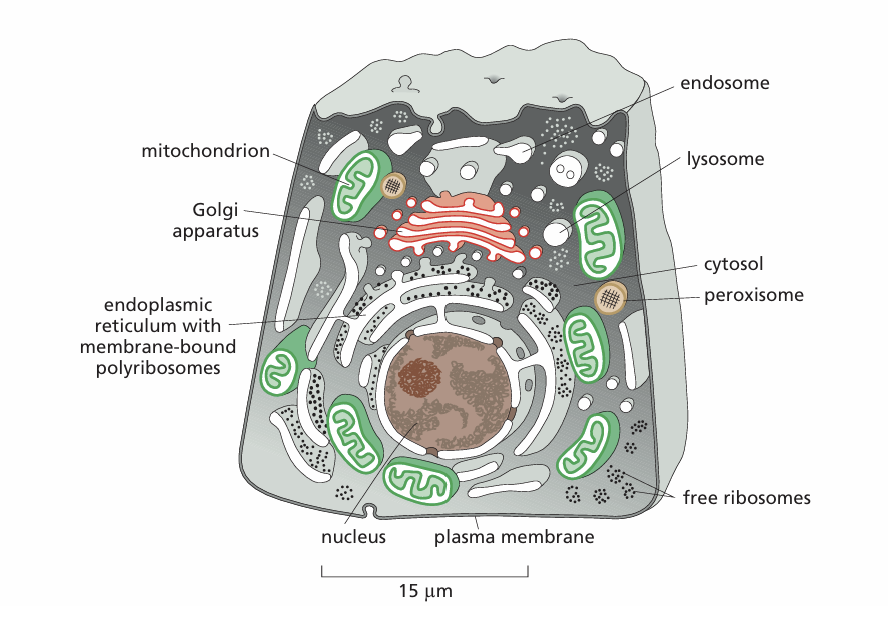
\includegraphics[width=0.5\linewidth]{compartmentOverview.png}
    \caption{overview of compartments}
    \label{fig:enter-label}
\end{figure}
    Compartamentalization in eukaryotic cells is used to improve metabolic process by providing optimal conditions for various reactions (such as very acidic conditions in lysosomes or very high calcium concentrations). In general this is achieved by having organelles.
    \par
    \textbf{Cellular compartments differ in function, form, subcellular location, protein and lipid coposition.} Moreover the may differ in ionic composition, e.g: pH can vary from 7.2 in the ER to less then 5 in lysosomes; Calcium concentration varries from nM in the cytoplasma to uM in the ER; The redox potential differs from reducing in the cytoplasm to oxidizing in the ER
    \par
    There are two types of organelles: \textbf{mebrane organelles and membrane-less organelles}

    \textbf{How many organelles?}

    \begin{itemize}
        \item 1 nucleous
        \item 1 golgi apparatus
        \item 1 ER
        \item hundreds of endosomes/lysosomes
        \item a mitochondrial network that is not always continous 
        \item memrbaneless organelles 
        
    \end{itemize}

   \textbf{ The number of organelles is not correlated with the size of the cell}. 

   This is very general and of course there are \textbf{exception }such as muscle cells and red blood cells. Muscle fiber are a fusion of many cells so they will have\textbf{ multiple nucleouses. } Wherease red blood cells will lose all internal membrane during differenciation so they will have\textbf{ no organelles that have a membrane}

  \paragraph{table on volumes of mebrane and organelles}

  \begin{figure}[H]
      \centering
      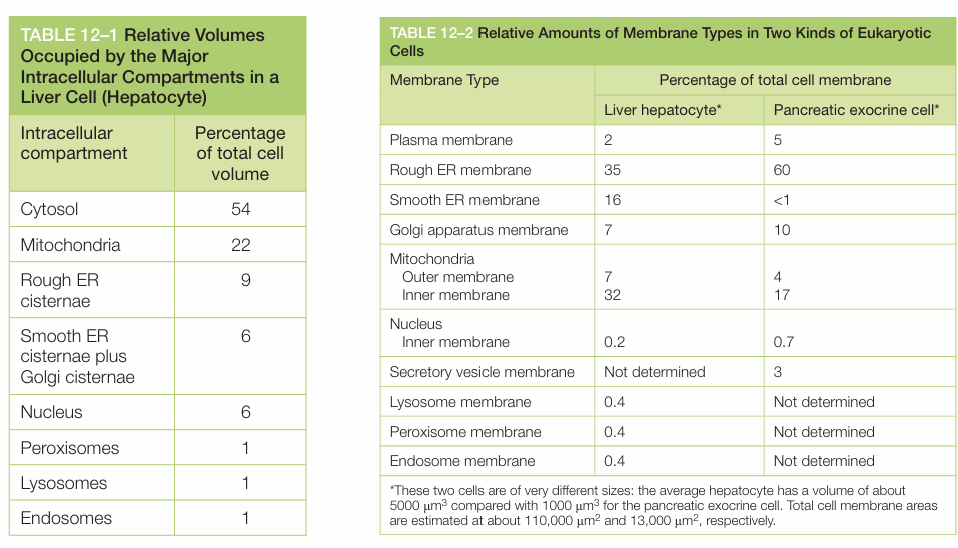
\includegraphics[width=\linewidth]{TableVolumes.png}
      \caption{table volumes of membranes}
      \label{fig:enter-label}
  \end{figure}

\begin{table}[h!]
\centering
\begin{tabular}{|l|l|}
\hline
\textbf{Membrane Organelles} & \textbf{Membrane-less Compartments} \\
\hline
Endoplasmic Reticulum             & \gls{P-bodies}                             \\
Nucleus                           & \gls{StressGranules}                      \\
Golgi System                      & Nucleolus                            \\
Peroxisomes                       & Many more to be discovered?          \\
Mitochondria                      &                                      \\
Lysosome                          &                                      \\
Endosome                          &                                      \\
\hline
\end{tabular}
\caption{Examples of membrane and membrane-less compartments in eukaryotic cells}
\end{table}

Membrane-less organelles are a rather new discovery but they usually require \textbf{\gls{LLPS}}. They can consist of protein aggregates or RNA aggregates, a similar principle is responsible for lipid raft formation:
\begin{figure}[H]
    \centering
    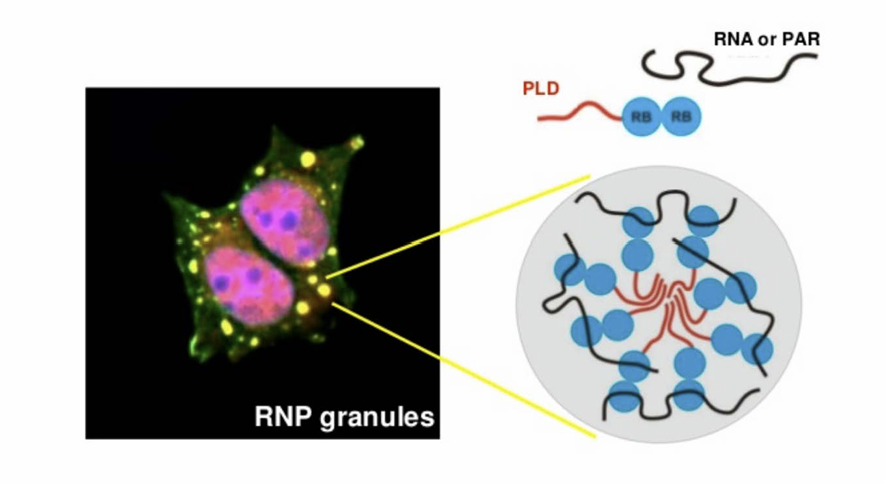
\includegraphics[width=0.5\linewidth]{RNP.png}
    \caption{membrane less organelle overview of \gls{RNP} }
    \label{fig:enter-label}
\end{figure}


\subsubsection{Endoplasmatic reticulum}
\begin{figure}[H]
    \centering
    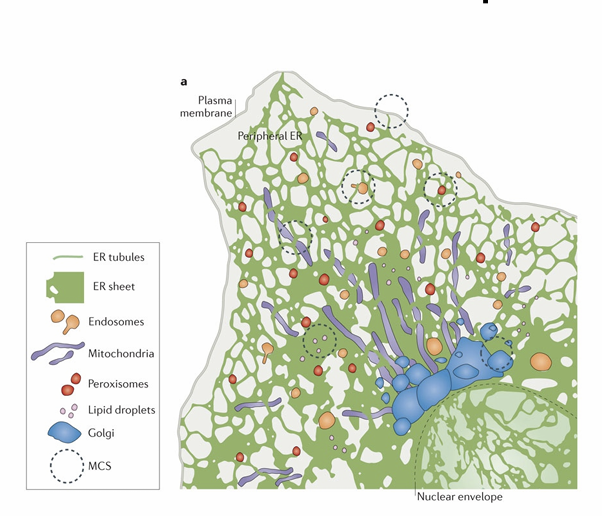
\includegraphics[width=0.5\linewidth]{ER.png}
    \caption{Structure of Endoplasmatic reticulum}
    \label{fig:enter-label}
\end{figure}
The \gls{EndoplasmicReticulum} is the \textbf{production site of all transmembrane proteins and lipids } it also serves as a \textbf{calcium storage of the cell}. The calcium is imported into the ER by the \textbf{\gls{SERCA}} There are two types of ER \textbf{smooth and rough ER}. The difference being that the \textbf{rough ER has membrane bound ribosomes} and the smooth one does not. Most cells will have both but the ratio will be different depending on cell type.

\paragraph{Smooth and rough ER separatation}
\begin{figure}[H]
    \centering
    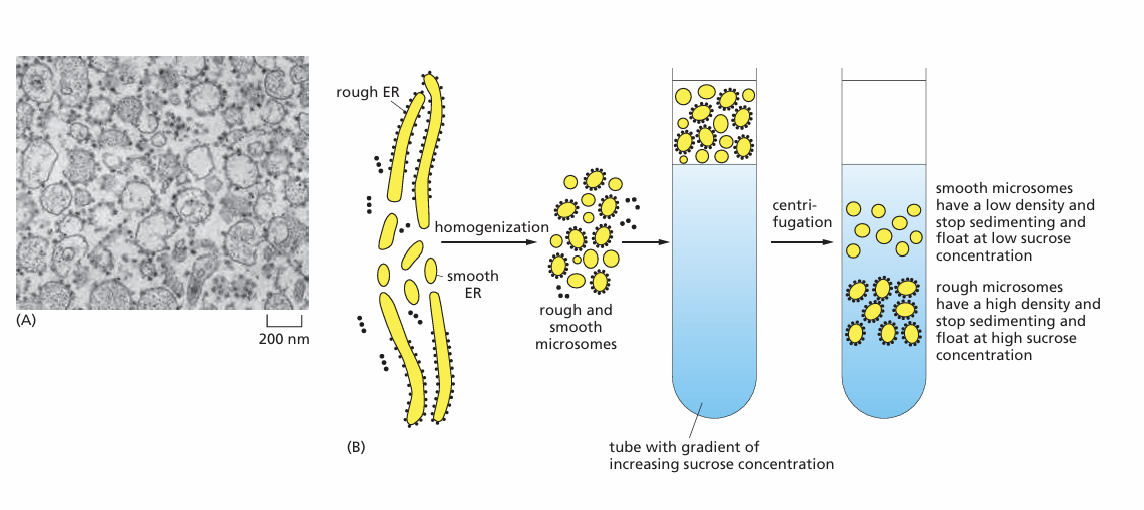
\includegraphics[width=0.5\linewidth]{ERSeparation.png}
    \caption{ER separation experiment}
    \label{fig:enter-label}
\end{figure}

Since smooth and rough ER have different densities they can be separated using a sucrose gradient and centrifugation. Here is how the process works:
\begin{enumerate}
    \item \textbf{Cell Lysis:} Cells are lysed using mechanical disruption (e.g., homogenization) or chemical methods to release cellular contents, including organelles and membrane fragments.
    
    \item \textbf{Differential Centrifugation:} The lysate is subjected to sequential centrifugation steps to remove nuclei and large organelles. The remaining supernatant is centrifuged at high speed to pellet \textbf{microsomes}, which are small vesicles derived from fragmented endoplasmic reticulum membranes.

    \item \textbf{Preparation of Sucrose Gradient:} A discontinuous or continuous sucrose gradient is prepared, typically ranging from 0.25~M to 2.0~M sucrose, to separate membrane vesicles based on density.

    \item \textbf{Loading of Microsomes:} The microsomal pellet is resuspended and carefully layered onto the sucrose gradient.

    \item \textbf{Ultracentrifugation:} The sample is centrifuged at high speed (e.g., 100{,}000~$\times$~g) for several hours. Microsomes migrate within the gradient according to their buoyant densities.

    \item \textbf{Fraction Collection:} Distinct layers form in the gradient: \textbf{rough ER-derived microsomes} (containing ribosomes) settle at higher density positions than \textbf{smooth ER-derived microsomes}, which are lighter. These fractions are collected separately.

    \item \textbf{Analysis:} Isolated ER fractions can be analyzed using protein assays, Western blotting, enzymatic activity tests, or proteomic approaches to study their composition and function.
\end{enumerate}





\subsubsection{Golgi system}
\begin{figure}[H]
    \centering
    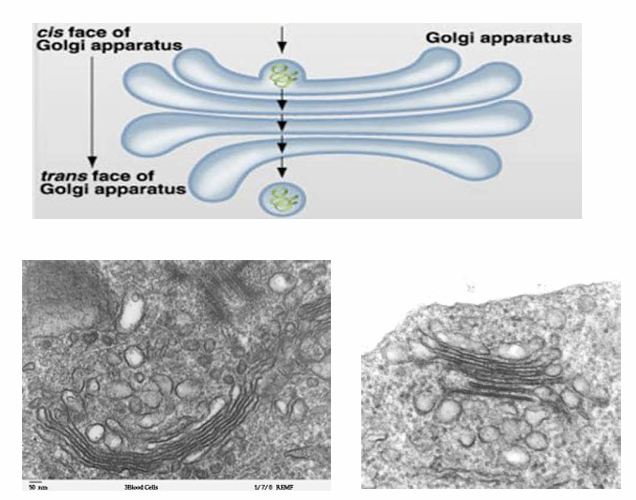
\includegraphics[width=0.5\linewidth]{Golgi.png}
    \caption{Glogi apparatus overview}
    \label{fig:enter-label}
\end{figure}

The Golgi apparatus acts as a \textbf{collection and dispatch center for proteins from the ER}. Proteins are packaged into vesicles, which fuse with the Golgi for further processing, mainly through\textbf{ post-translational modifications such as glycosylation and phosphorylation.} These modifications help direct proteins to their final destination.
\begin{figure}[H]
    \centering
    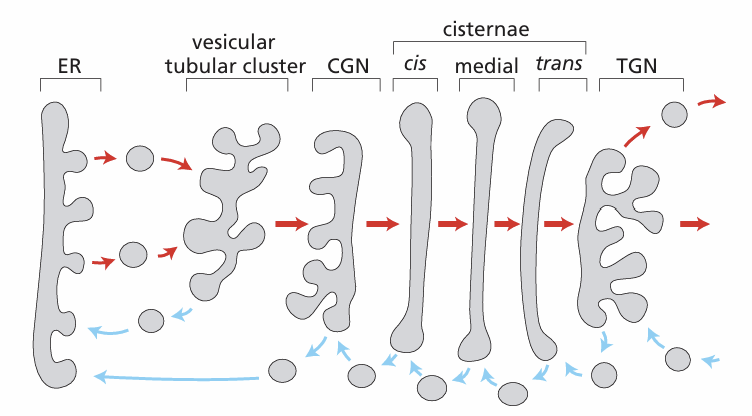
\includegraphics[width=0.5\linewidth]{GolgiParts.png}
    \caption{domains of the golgi}
    \label{fig:enter-label}
\end{figure}
The golgi can be further subdivided into domains (breif chaptGPT overview of these):
\begin{itemize}
    \item \textbf{Cis-Golgi Network (CGN):} The entry face of the Golgi apparatus, located closest to the endoplasmic reticulum (ER). It receives proteins and lipids from the ER and is involved in initial processing, such as phosphorylation and sorting for further transport or ER retrieval.

    \item \textbf{Medial-Golgi:} The central region of the Golgi stack. It performs further modification of glycoproteins, including the processing of N-linked oligosaccharides and initiation of O-linked glycosylation.

    \item \textbf{Trans-Golgi:} The portion closer to the exit side of the Golgi. It completes final processing steps like sulfation and complex glycosylation, preparing molecules for sorting.

    \item \textbf{Trans-Golgi Network (TGN):} A dynamic sorting compartment at the trans face of the Golgi. It directs modified proteins and lipids to their final destinations, including the plasma membrane, lysosomes, or secretory vesicles, using different types of transport vesicles.
\end{itemize}


\subsubsection{lysosomes}
\begin{figure}[H]
    \centering
    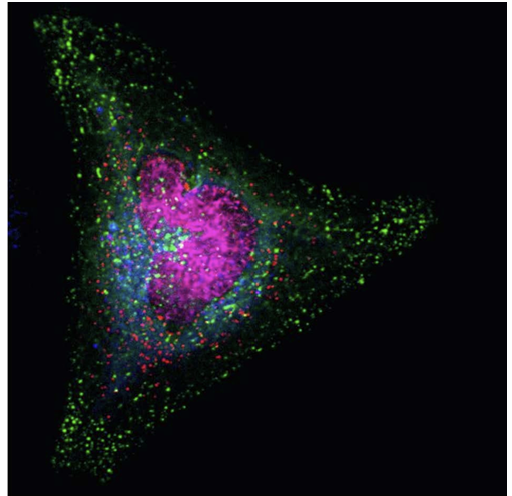
\includegraphics[width=0.3\linewidth]{lysosome.png}
    \caption{lysosome fluorecent microsopy image}
    \label{fig:enter-label}
\end{figure}
lysosomes are specialized vesicles with very low ph (4.5-5) they house \textbf{a multitidue of enzymes} that require these conditions such as enzymes involved in\textbf{ lysis} of peptides nucleic acids carbohydrates and lipids. \textbf{They contain more than 60 enzymes and more than 50 membrane proteins and highly variable in size}


\subsubsection{Mitochondria}
\begin{figure}[H]
    \centering
    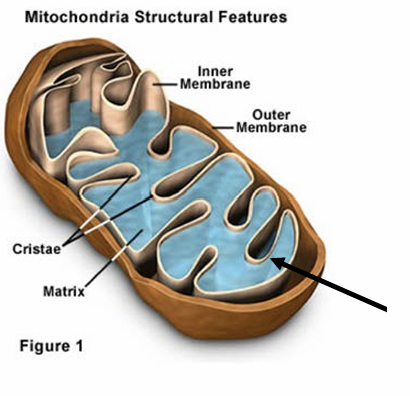
\includegraphics[width=0.5\linewidth]{mitochondria.png}
    \caption{Mitochondra structure}
    \label{fig:enter-label}
\end{figure}
The \textbf{mitochonria is a double mebraned organelle}. This is due to the fact that it is an ex. bacteria that the cell tried to eat but fucked up. However now it can't survive outside of the cell. 

\subsubsection{Endosomes}
\begin{figure}[H]
    \centering
    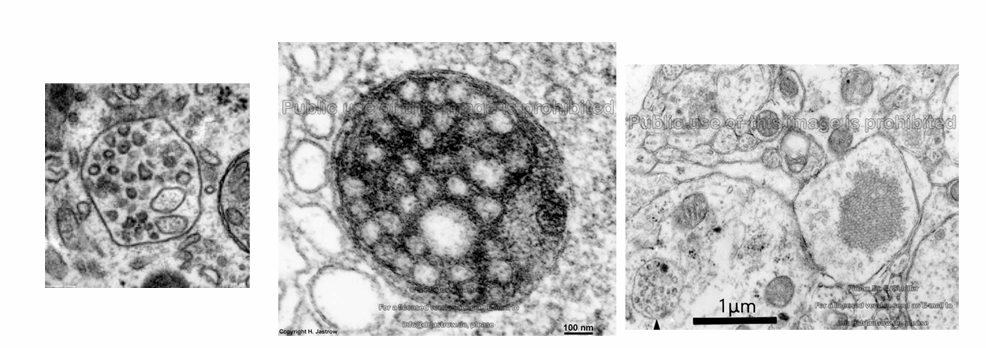
\includegraphics[width=0.5\linewidth]{endosomes.png}
    \caption{Endosomes}
    \label{fig:enter-label}
\end{figure}
Endosomes are a \textbf{collection of intracellular sorting organelles in eukaryotes} (there was literally nothing else here...)

\subsubsection{Peroxysomes}
\begin{figure}[H]
    \centering
    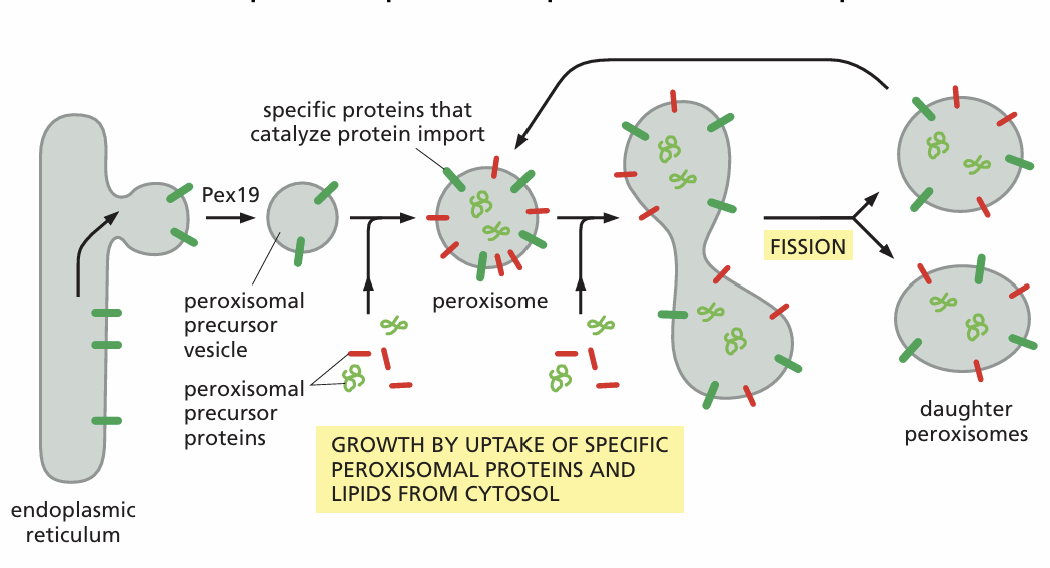
\includegraphics[width=\linewidth]{Peroxy.png}
    \caption{Peroxysomes proliferation}
    \label{fig:enter-label}
\end{figure}
Peroxysomes are specialized vesicle that is used to \textbf{peroxidize shit}. (hence the name) Usually it's substrates are toxins that come from the liver or the kindey cells. The reaction is as follows:
\begin{equation}
\mathrm{H_2O_2} + \mathrm{R'H_2} \rightarrow \mathrm{R'} + 2\mathrm{H_2O}
\end{equation}

They are created from the ER first as a \textbf{peroxisomal precursor vesicle} These then fuse with \textbf{peroxisomal precursor proteins and lipids}. (these are found in the cytosol) forming the main peroxisome that can then fission to produce more peroxysomes. They are also responsible for the \textbf{break down of fatty acids}, however unlike \gls{BetaOxidation} it isn't ATP coupled. 


\subsubsection{lipid droplets}
\begin{figure}[H]
    \centering
    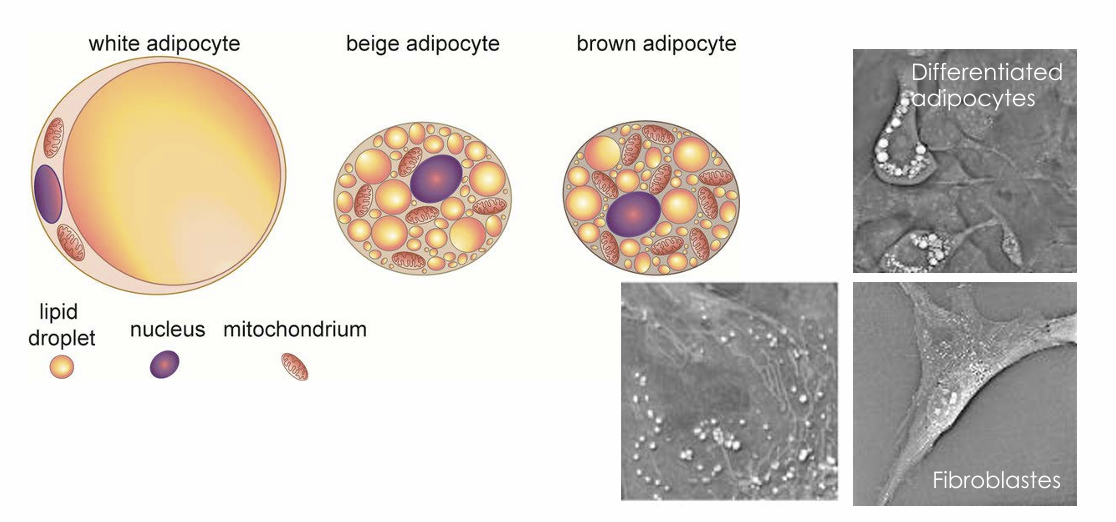
\includegraphics[width=0.5\linewidth]{fatCells.png}
    \caption{adipocyte overview}
    \label{fig:enter-label}
\end{figure}

These are specialized cells that store lipid droplets. Note that\textbf{ white adipocytes are mainly used for storage} hence the oversized lipid droplet, whereas \textbf{brown adipocytes are used for heat generation}, which is why they have a lot of mitrochondia

\subsection{lipid composition of various organelles}
The lipid composition is different across the various organelles. 
\begin{figure}[H]
    \centering
    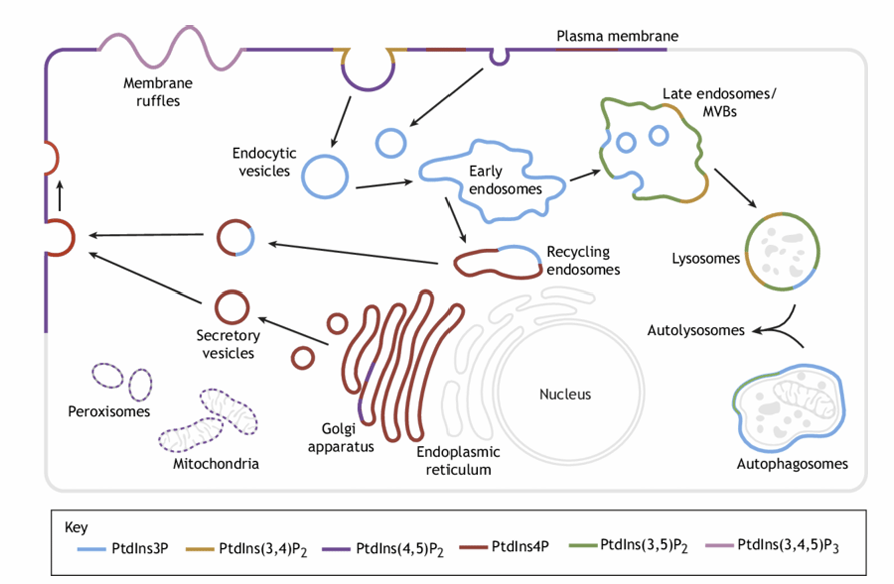
\includegraphics[width=\linewidth]{PI_overview.png}
    \caption{Phosphatidylinositols location and phosphorylation state}
    \label{fig:enter-label}
\end{figure}
An interesting case is that of PI, which depending on the\textbf{ cellular location will be phosphorylated differently}

The composition of the cell mebrane will also vary across cell types. This is illustrated in the table below:
\begin{figure}[H]
    \centering
    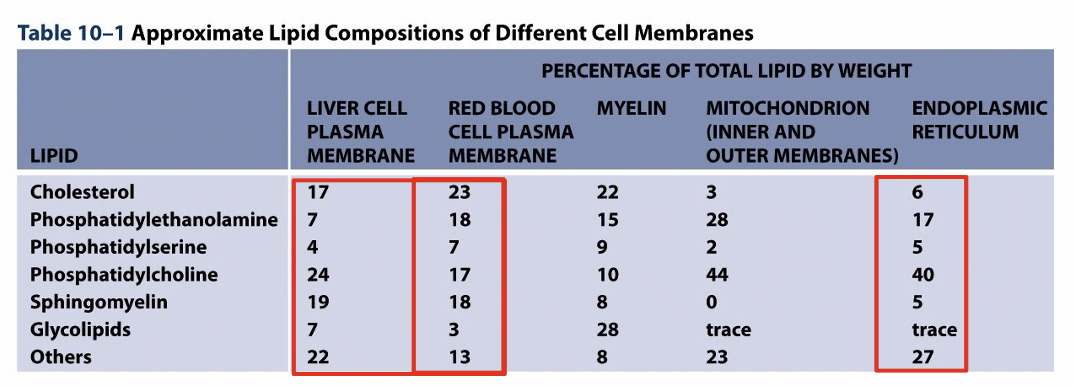
\includegraphics[width=\linewidth]{Mebranecomposition.png}
    \caption{Membrane composition based on cell type}
    \label{fig:enter-label}
\end{figure}


\subsection{protein localization}
\subsubsection{types of transport}


\begin{figure}[H]
    \centering
    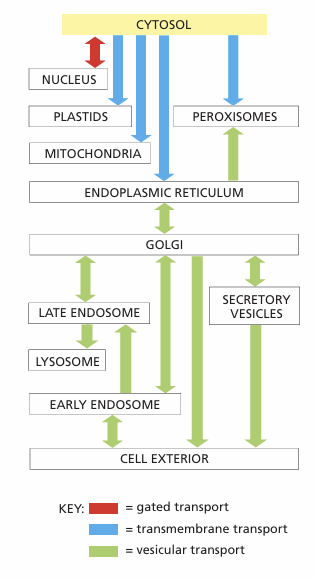
\includegraphics[width=0.3\linewidth]{typesOfTransport.png}
    \caption{Types of transport overview}
    \label{fig:enter-label}
\end{figure}
There are three types of \textbf{transport Gated, transmembrane localization, vesicular transport}:

\begin{enumerate}
    \item \textbf{gated transport}: In gated transport, proteins and RNA molecules move between the 
cytosol and the nucleus through \textbf{nuclear pore complexes} in the nuclear envelope. The 
nuclear pore complexes function as \textbf{selective gates} that support the active transport of 
specific macromolecules and macromolecular assemblies \textbf{between the two topologically 
equivalent spaces}, although they also allow free diffusion of smaller molecules

\item \textbf{Transmembrane localisation}: In protein translocation, transmembrane protein 
translocators directly transport specific proteins across a membrane from the cytosol 
into a \textbf{space that is topologically distinct}. The transported protein molecule usually must 
unfold to snake through the \textbf{\gls{translocators}}. The initial transport of selected proteins from 
the cytosol into the ER lumen or mitochondria, for example, occurs in this way. Integral 
membrane proteins often use the same translocators but translocate only partially 
across the membrane, so that the protein becomes embedded in the lipid bilayer.

\item \textbf{vesicular transport} in Vesicular transport, membrane-enclosed transport 
intermediates— which may be small, spherical transport vesicles or larger, irregularly 
shaped organelle fragments—ferry proteins from\textbf{ one topologically equivalent 
compartment to another}. This involves the creation of vesicles where the mebrane proteins are loaded onto. These then are ferried around and fuse with another compartment.

\end{enumerate}

\subsubsection{important signals}
\begin{figure}[H]
    \centering
    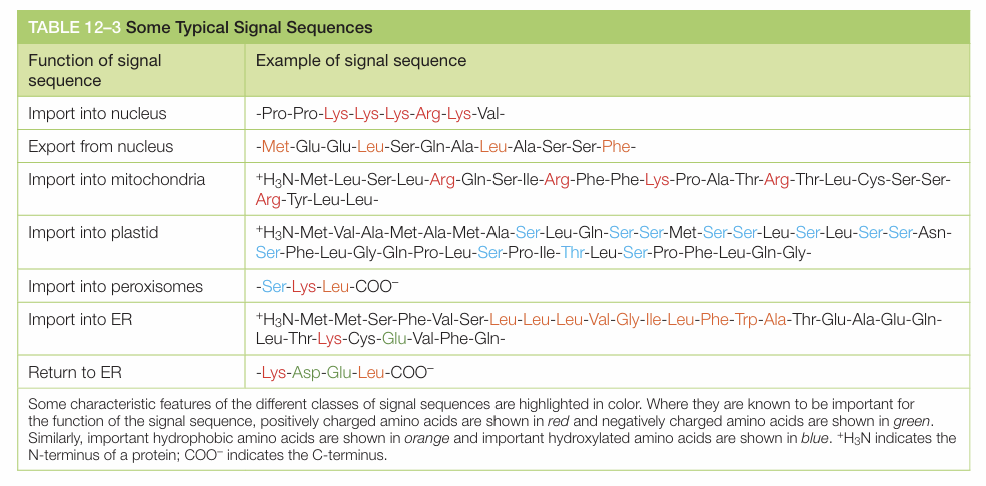
\includegraphics[width=\linewidth]{ImportantSignals.png}
    \caption{list of important localization signals}
    \label{fig:enter-label}
\end{figure}
Note that the signals can be either N or C terminal.\textbf{ N-terminal signals are read during translatio, where as C-terminal tags are read post-translationally}. The \textbf{nuclear export signals can be in the middle of the CDS}. Note also that most of the localization signals will be cut off after their use, with exceptions such as nuclear localization tag (\gls{NLS}) and Peroxisomal targeting signal

\subsubsection{nuclear import}


\begin{figure}[H]
    \centering
    % First subfigure (side by side)
    \subfigure[Nuclear pore complex]{
        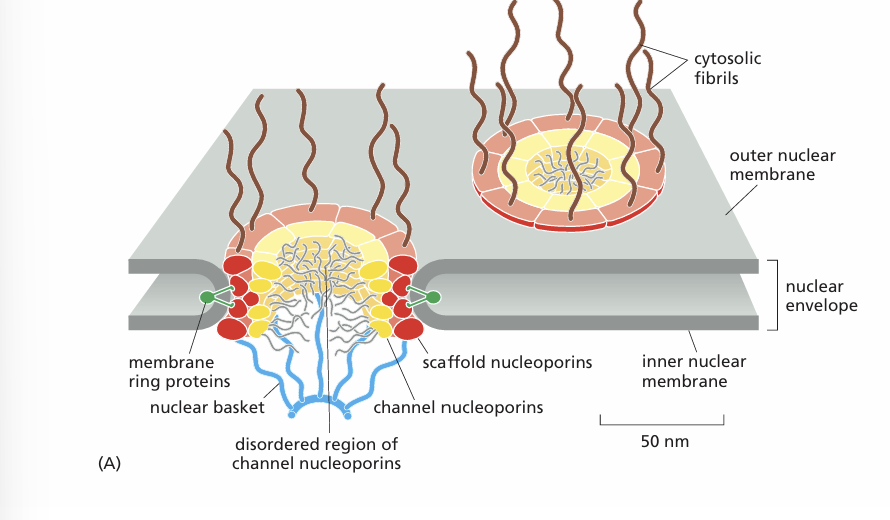
\includegraphics[width=0.65\linewidth]{NPC.png}
        \label{fig:itc}
    }
    \hspace{0.05\textwidth} % Adds a small horizontal space between the figures
    % Second subfigure (side by side)
    \subfigure[nucleus structure]{
        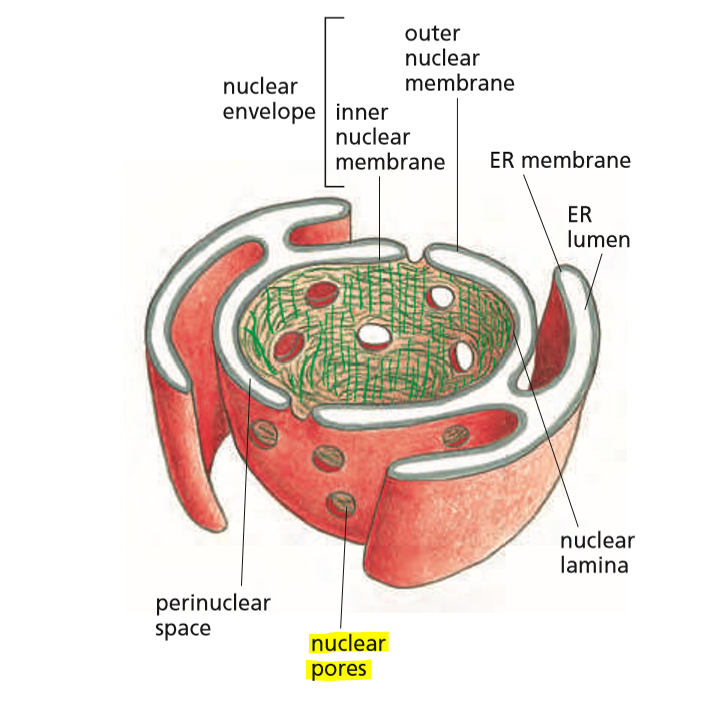
\includegraphics[width=0.25\linewidth]{NucleusStructure.png}
        \label{fig:ITC_H_L}
    }
    \caption{Application of protein design}
    \label{fig:ITC_all}
\end{figure}

The nuclear import is special as it requires the molecule to pass through the \textbf{nuclear pore complexes (\gls{NPC})} which are giant channels in the nuclear membrane that \textbf{regulate traffic into the nucleous.}  The nuclear pores \textbf{allow any protein less than 5kDa and ions to pass freely.} Another thing to note is that the nuclear pore complexes \textbf{regulates traffic in both ways, and is unclear how it does this as to avoid crashes}

\paragraph{Ribosome production example}

\begin{figure}[H]
\centering
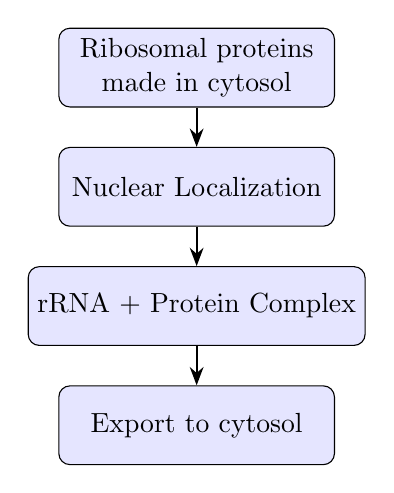
\begin{tikzpicture}[
  node distance=0.5cm and 1cm,
  every node/.style={align=center},
  process/.style={rectangle, draw, rounded corners, minimum width=3.5cm, minimum height=1cm, fill=blue!10},
  arrow/.style={-{Stealth}, thick}
]

% Nodes
\node[process] (cytosol) {Ribosomal proteins\\ made in cytosol};
\node[process, below=of cytosol] (nucleus) {Nuclear Localization};
\node[process, below=of nucleus] (complex) {rRNA + Protein Complex};
\node[process, below=of complex] (export) {Export to cytosol};

% Arrows
\draw[arrow] (cytosol) -- (nucleus);
\draw[arrow] (nucleus) -- (complex);
\draw[arrow] (complex) -- (export);


\end{tikzpicture}
\caption{Overview of Ribosome Production and Trafficking}
\end{figure}
Ribosomes are \textbf{made in the cytosol} then \textbf{imported into the nucleus } where they complex with rRNA's. Then they are \textbf{exported back out} of the nucleous

\paragraph{Nuclear import receptors(importins)}
\begin{figure}[H]
    \centering
    % First subfigure (side by side)
    \subfigure[Nuclear import protein]{
        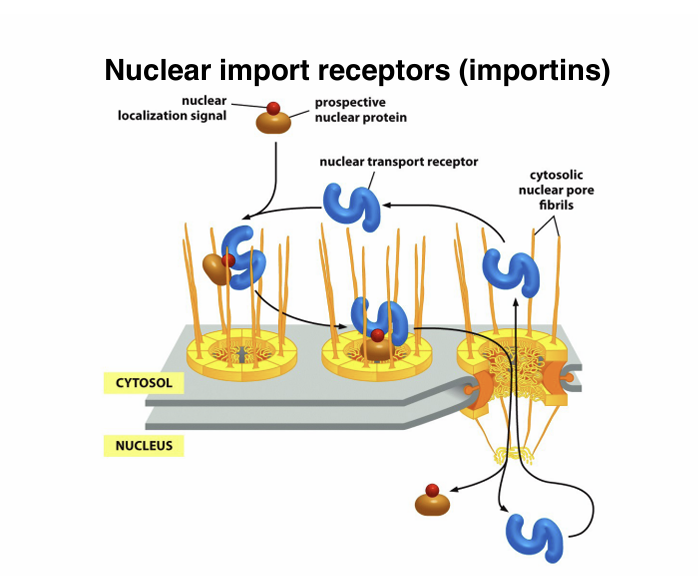
\includegraphics[height=4cm]{importins.png}
        \label{fig:itc}
    }
    \hspace{0.05\textwidth} % Adds a small horizontal space between the figures
    % Second subfigure (side by side)
    \subfigure[Nucleus structure]{
        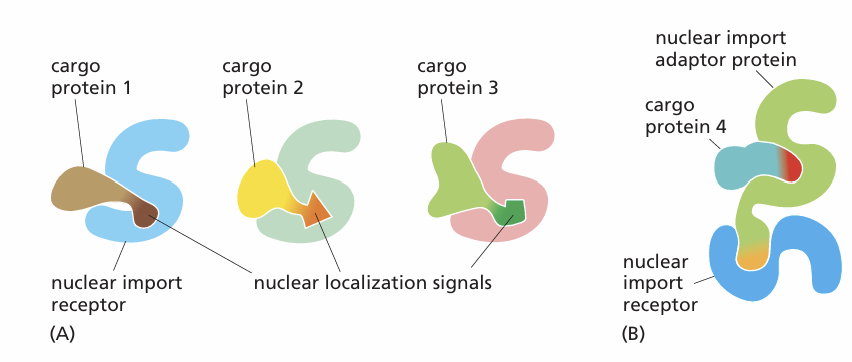
\includegraphics[height=4cm]{CargoProteins.png}
        \label{fig:ITC_H_L}
    }
    \caption{Importins bind to cargo proteins that have NLS}
    \label{fig:ITC_all}
\end{figure}





Proteins destined for the nucleus need to be shuttled into it by the \textbf{nuclear import receptors (\gls{importin}) that bind to the localiztion signal on the cargo protein} The localization signals is \textbf{not found on the N or C terminus and are not cut off.} This is due to the fact that they need to be\textbf{ used everytime the nucleus is reformed after cell division.}
Nuclear import receptors (importins) are \textbf{tightly linked to a GTPase cycle}, specifically involving the small GTPase Ran

\subparagraph{ran-GDP Ran-GTP}

\begin{figure}[H]
    \centering
    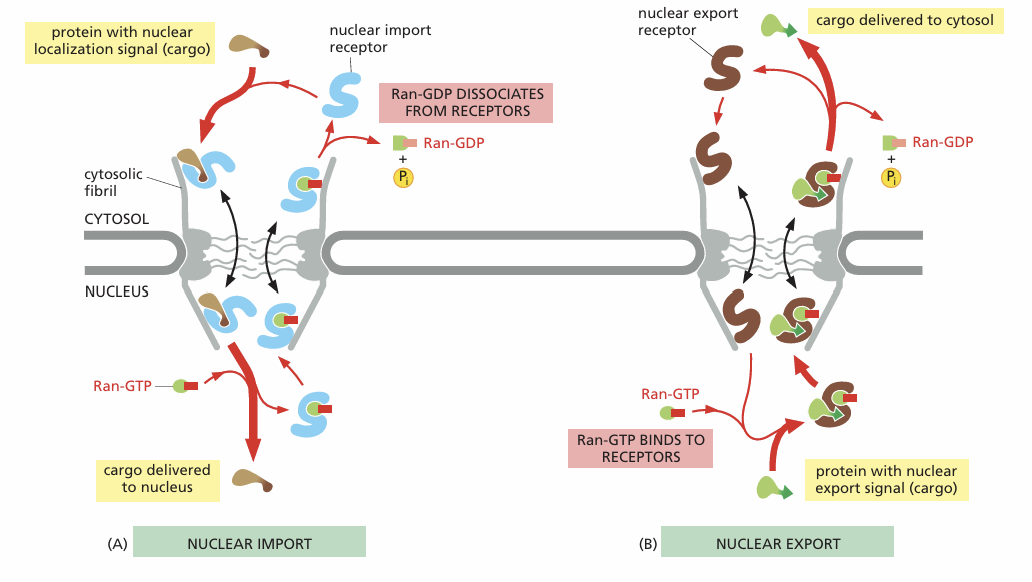
\includegraphics[width=\linewidth]{RanGDP.png}
    \caption{ran-GDP ran-GTP and it's role in shuttling cargo across nuclear pore complexes}
    \label{fig:enter-label}
\end{figure}

Ran-GTP is primarily found inside nucleus due to presence of \textbf{(\gls{gef}}. Ran-GDP is found in the cytosol due to presence of \textbf{\gls{gap}}. The \textbf{Ran-GPT/GDP works as a molecular switch} which allows regulation of directionality of nuclear import and export.
\begin{itemize}
    \item \textbf{Nuclear Import}
    \begin{enumerate}
        \item Cargo with nuclear localization signals binds to import receptors.
        \item The import receptor-cargo complex enters the nucleus through the nuclear pore.
        \item Ran-GTP binds to the import receptor, causing cargo release inside the nucleus.
        \item The Ran-GTP-import receptor complex is exported to the cytosol.
        \item Ran-GAP promotes GTP hydrolysis, converting Ran-GTP to Ran-GDP, leading to receptor release.
    \end{enumerate}
    
    \item \textbf{Nuclear Export}
    \begin{enumerate}
   
        \item Cargo with nuclear export signals binds to export receptors \textbf{(\gls{exportin})} in the nucleus.
        \item Ran-GTP binds to the export receptor-cargo complex.
        \item The complex exits the nucleus through the nuclear pore.
        \item In the cytosol, Ran-GAP promotes GTP hydrolysis, converting \gls{ranGTP} to \gls{ranGDP}.
        \item Cargo is released into the cytosol, and the export receptor is recycled.
    \end{enumerate}
\end{itemize}

\begin{remark}
    
\begin{figure}[H]
    \centering
    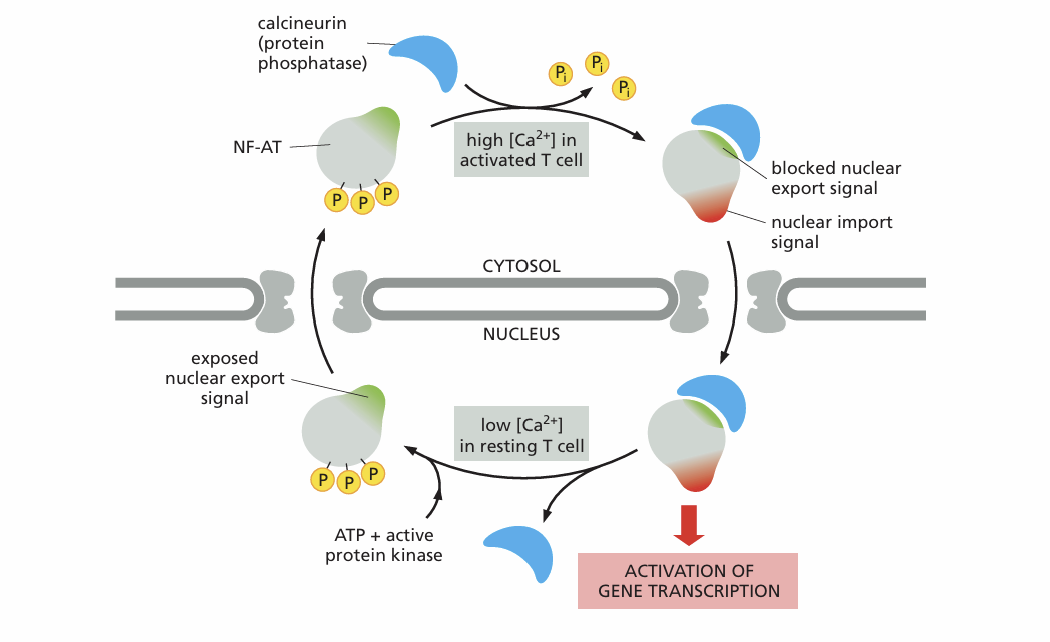
\includegraphics[width=0.7\linewidth]{TCells.png}
    \caption{role of nuclear import/ export signals in T cell activation}
    \label{fig:enter-label}
\end{figure}

Nuclear and import signals play a crucial role in T cell activation. \textbf{Upon activation the T-cell's cytosolic Ca2+ concetration will be very high.} (it usually is low, like all cells). This then triggers \textbf{\gls{calcineurin} to dephosphorylate the nuclear import signal and bind to the nuclear export signal.} this the moves th\textbf{e NF-AT (transcrition factor inside the nucleus} promoting gene expression needed for T-Cell activation.
\end{remark}



\paragraph{the role of nuclear import in cell division}
\begin{figure}[H]
    \centering
    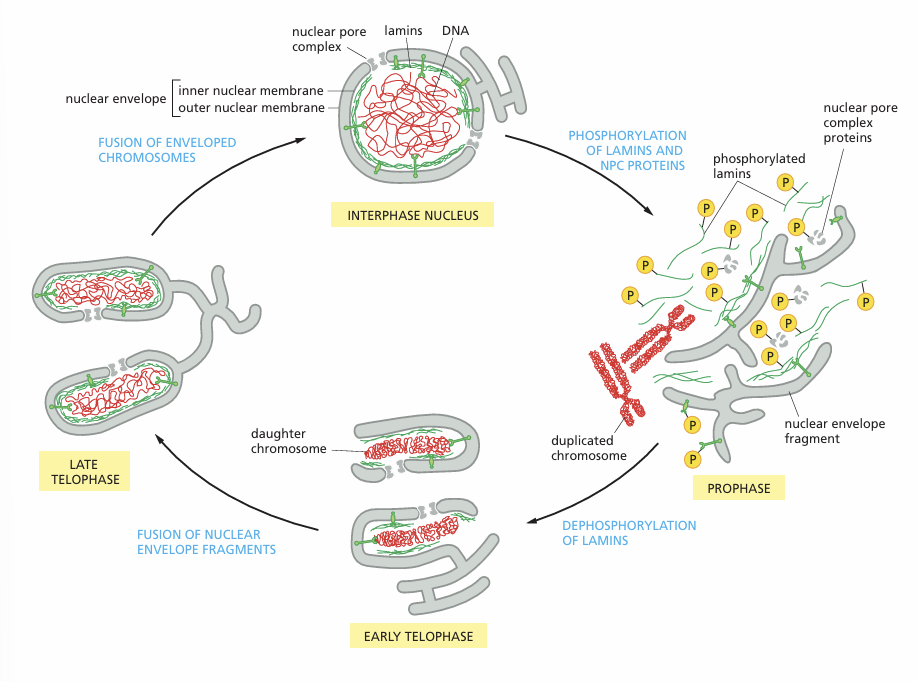
\includegraphics[width=0.7\linewidth]{NuclearReforming.png}
    \caption{Reformation of the nucleaus requires resusable NLS}
    \label{fig:enter-label}
\end{figure}
After the cell divides the Nuclear pore complexes are closed, as they are tighly bound to chromosomes. This means that \textbf{only proteins bound to mitotic chromosomes will be found inside the nucleus during cell division} cytosolic proteins are virtually excluded from the reforming the nucleus and will need to be \textbf{imported once the nuclear envelope is completed}


\subsubsection{main transport pathways for proteins}
There are two transport pathways in the cell that of \textbf{biosynthesis} and that of \textbf{endocytosis}
\begin{figure}[H]
    \centering
    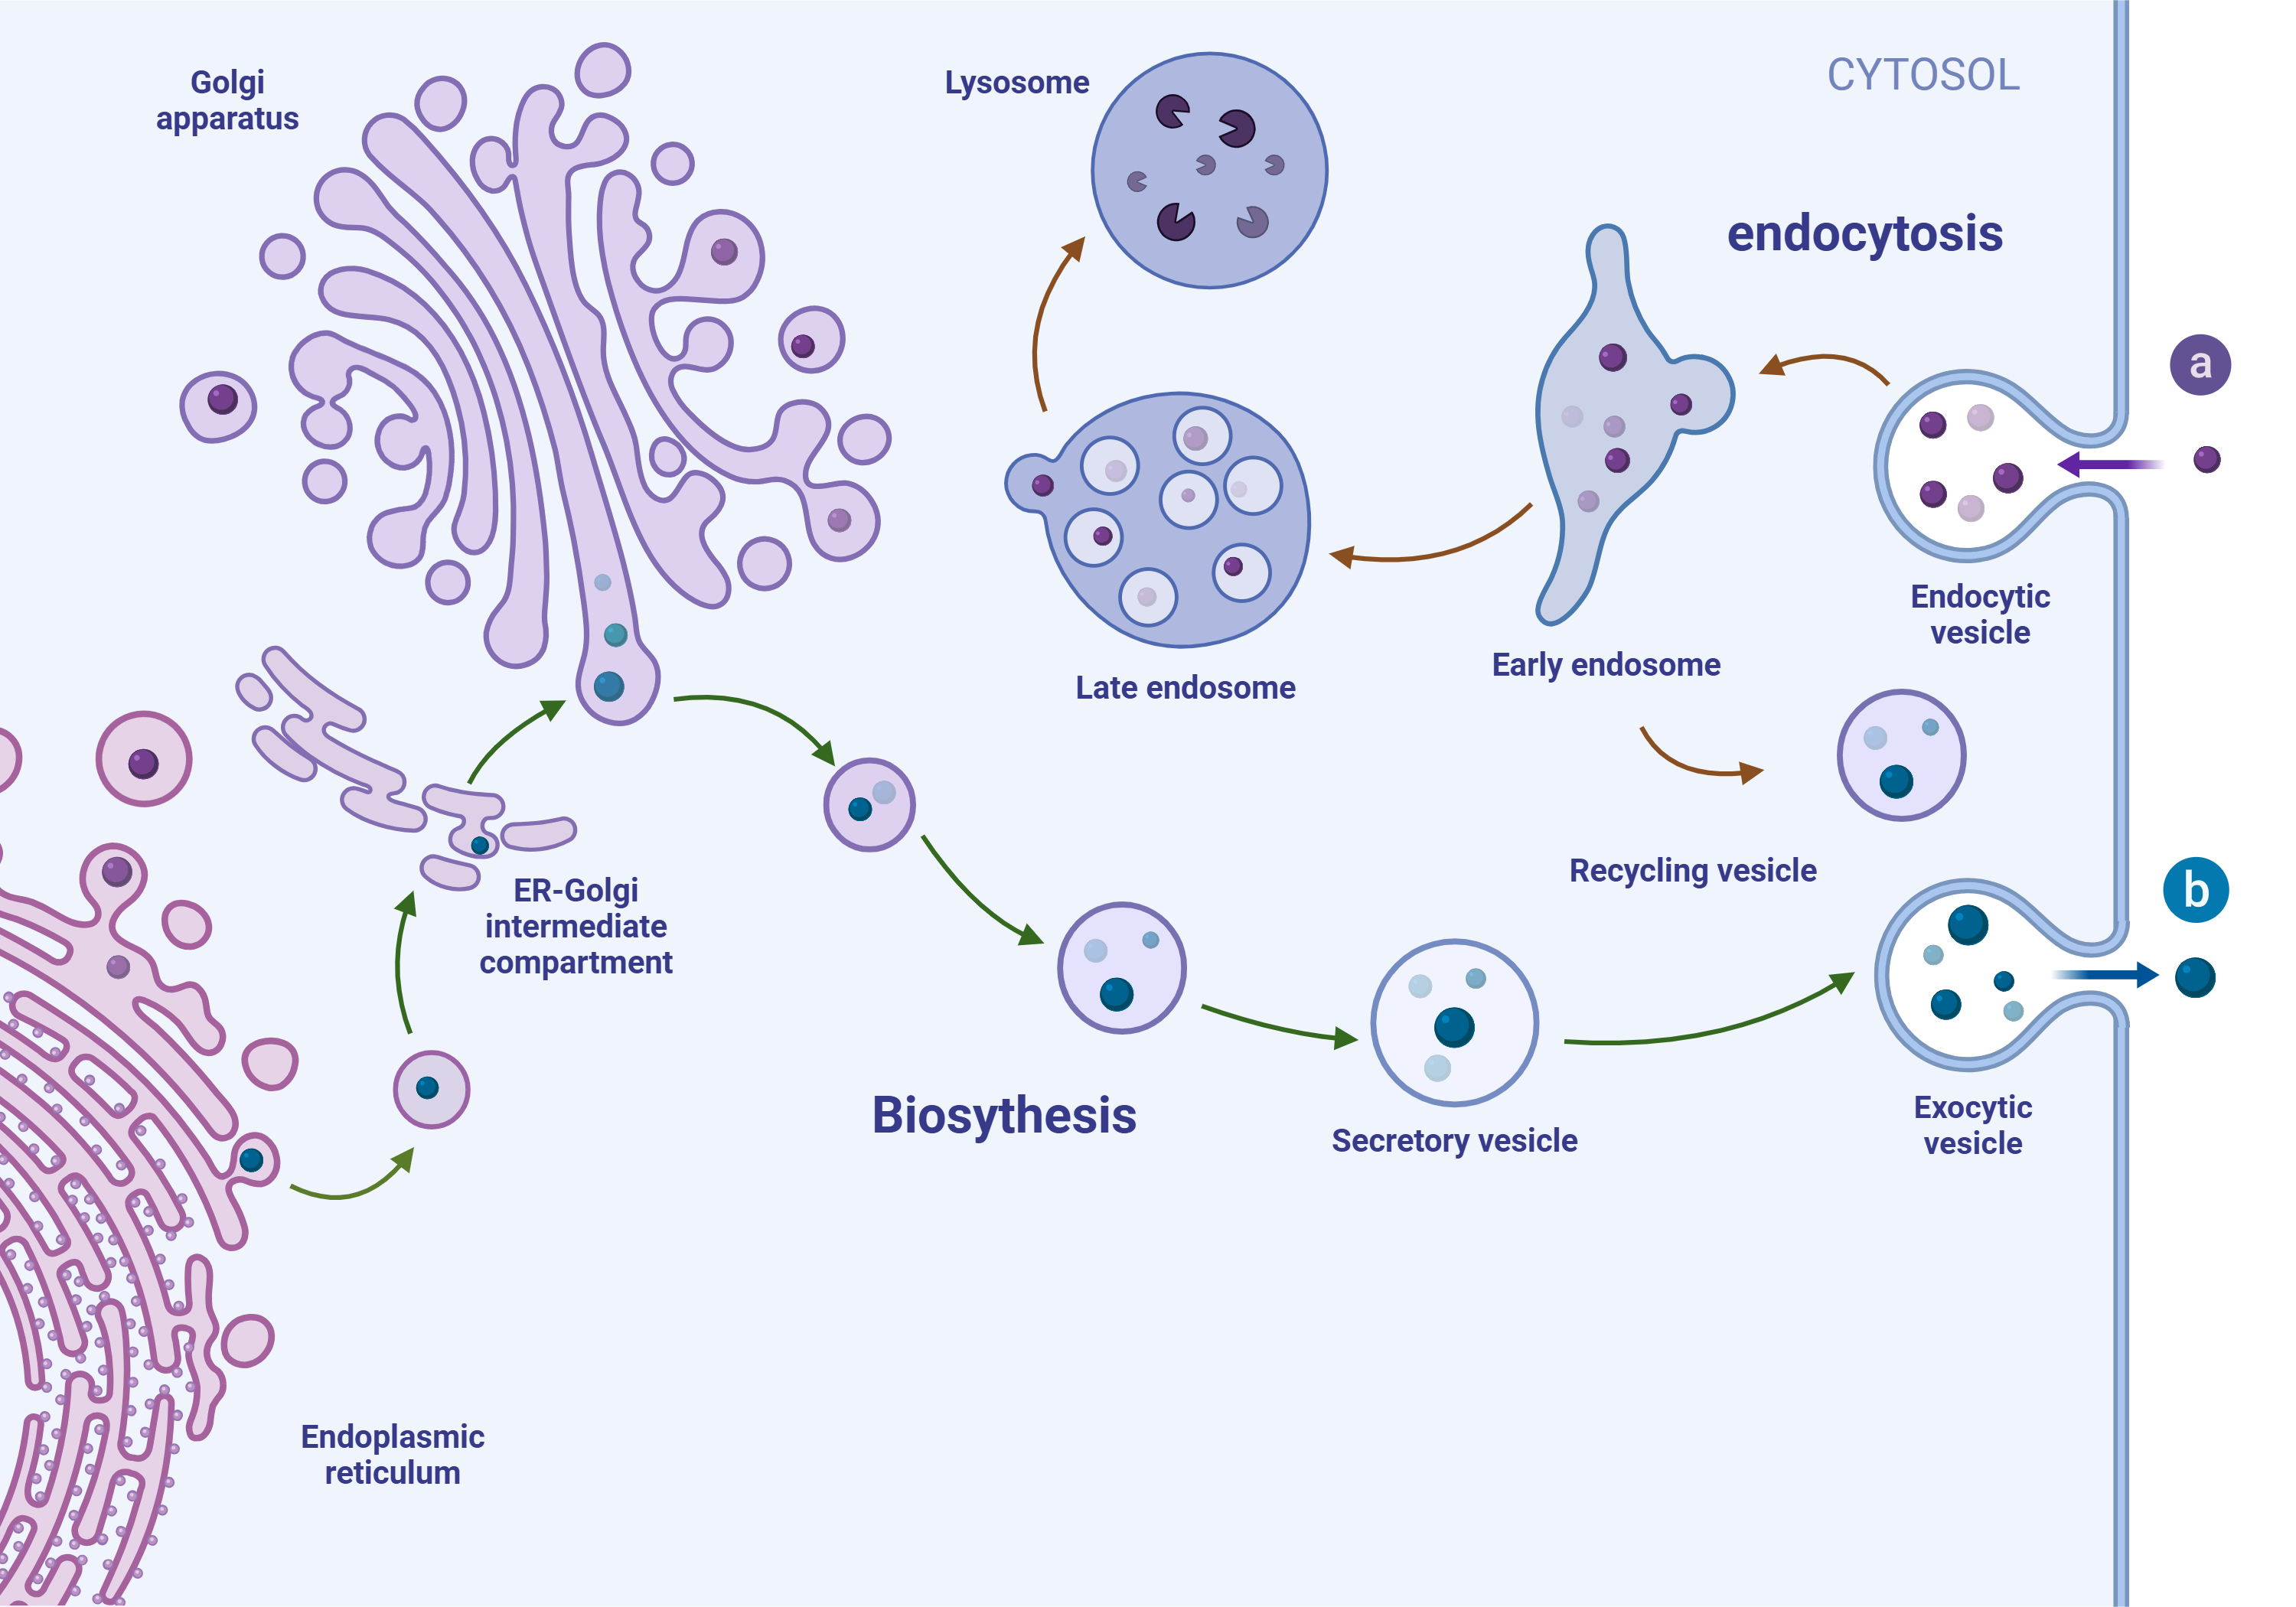
\includegraphics[width=0.7\linewidth]{Pathways (1).png}
    \caption{Main Pathways looked at in this chapter}
    \label{fig:enter-label}
\end{figure}
\textbf{Biosythesis}
\begin{enumerate}
    \item ER
    \item Golgi apparatus
    \item Trans Golgi network
    \item plasma membrane where vesicle fuses and proteins are secreted.
\end{enumerate}

\textbf{Endocytosis}
\begin{enumerate}
    \item uptake of proteins from \textbf{plasma membrane}
    \item \textbf{early endosomes}: here the cell has to decide wether to recyle the material taken up (such as receptors) or destroy it. if it recyles it it will become a recylcing endosome otherwise it will become a lysosome where the proteins will be digested and broken down into individual AA.
    \item  \textbf{recycling endosomes}: used for receptor reuptake. It will fuse with memrbane rexposing the receptors in the cell exterior.

    \item \textbf{late endosome} will eventuall convert to \textbf{lysosome } where the uptaken material will be digested
\end{enumerate}

\subsubsection{translocation to ER}

\paragraph{cotranslational and post translational localization}
\begin{figure}[H]
    \centering
    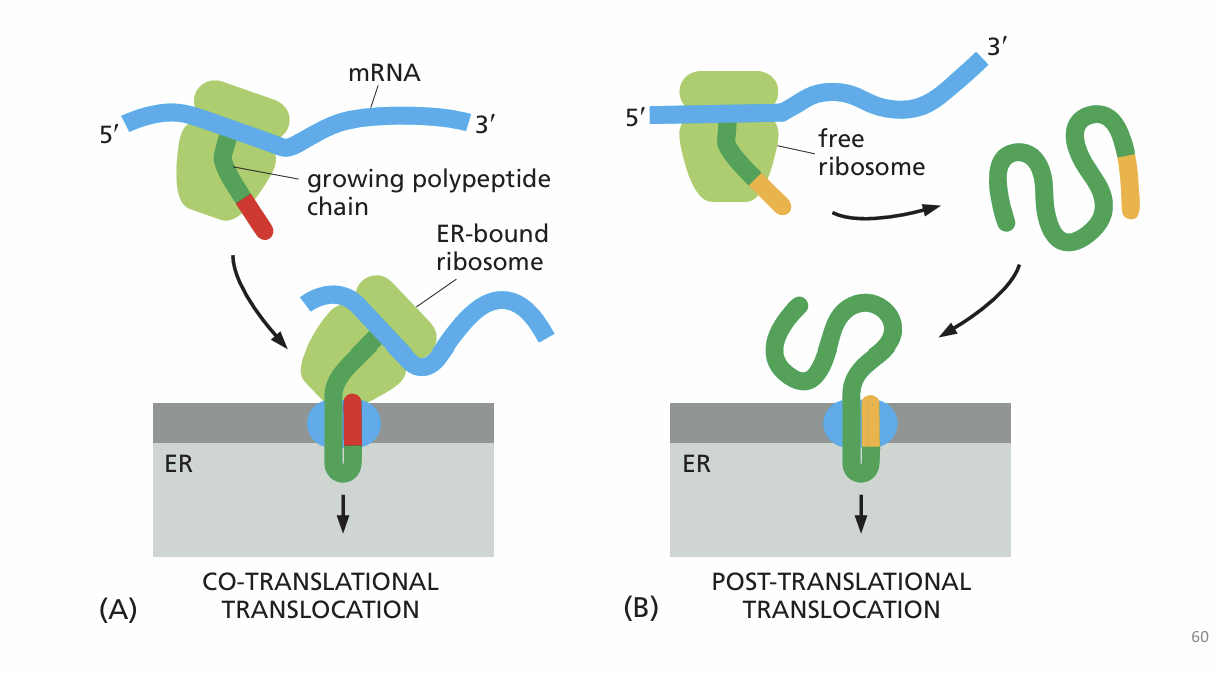
\includegraphics[width=0.7\linewidth]{CoTranslation.png}
    \caption{co and post translocation to the ER}
    \label{fig:enter-label}
\end{figure}

\textbf{\gls{cotranslocation}} involves the ribosome being moved to the ER as soon as the nacent protein's ER localization signal is produced. Then the signal peptide is\textbf{ cleaved off if the proteins is a ER lumen cytosolic protein.} \textbf{All memrbane proteins are cotranslational} Whereas \gls{postrtranslocation} involves the protein being localized to ER after it has been fully translated.


\paragraph{soluble proteins}

\textbf{Soluble proteins that are ER bound must have an ER localization signal.} Once in the ER Lumen the localization signal will be \textbf{cleaved off}. Note that the ER-Lumen is not a highly reducing enviroment like the cytosol. Thus ER cystosolic proteins can have disulfide bonds unlike cytosolic proteins.

\paragraph{transmembrane proteins}
\begin{figure}[H]
    \centering
    % First subfigure (side by side)
    \subfigure[single pass proteins]{
        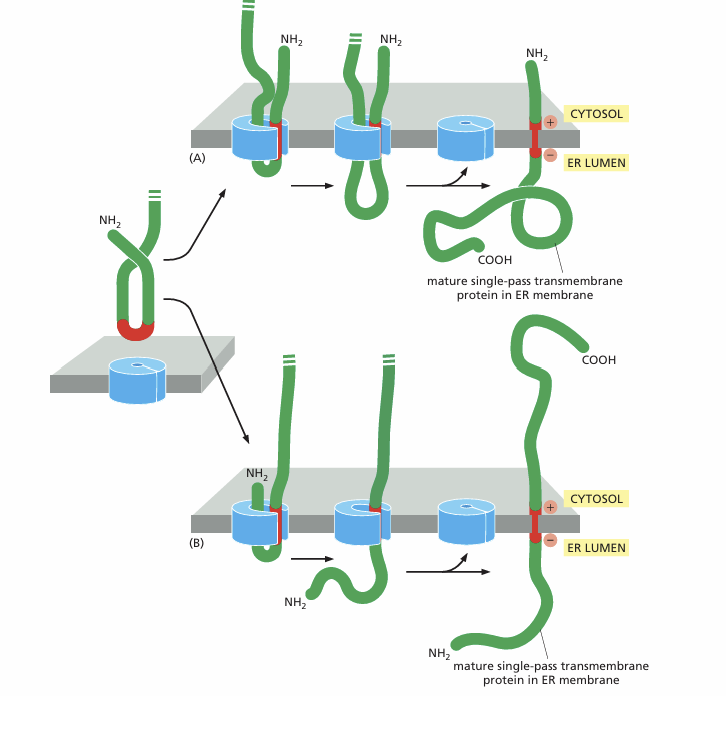
\includegraphics[height=6cm]{singlePassTransmembrane.png}
        \label{fig:itc}
    }
    \hspace{0.05\textwidth} % Adds a small horizontal space between the figures
    % Second subfigure (side by side)
    \subfigure[multipass proteins]{
        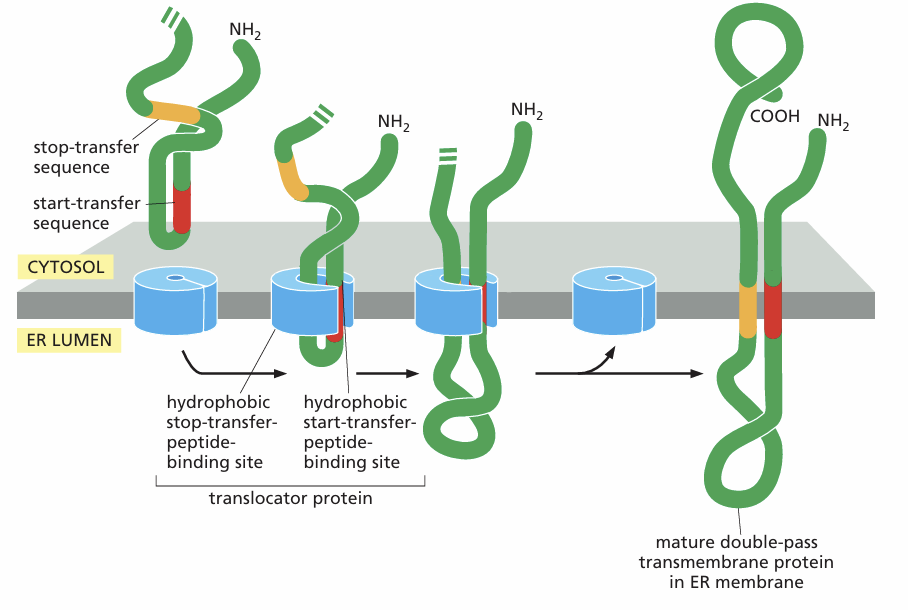
\includegraphics[height=6cm]{multiPass.png}
        \label{fig:ITC_H_L}
    }
    \caption{Role of localization in transmembrane protein translation}
    \label{fig:ITC_all}
\end{figure}
Transmembrane proteins are special in that they \textbf{need cotranslational traslocation into ER membrane} as otherwise they will not be embedded into membrane. As they are produced they will be funneld through translocator until a \textbf{start signal }is found which will create the transmembrane domain until the next \textbf{stop-transfer sequence } Unlike soluble proteins they also \textbf{don't necessarly need an N-terminal localization signal} when the N-terminus is cytoplasmic they can have an "internal" localization signal that won't be cut off at one of the transmembrane domains.

\subparagraph{the GPI anchor and tail anchored proteins}

\begin{figure}[H]
    \centering
    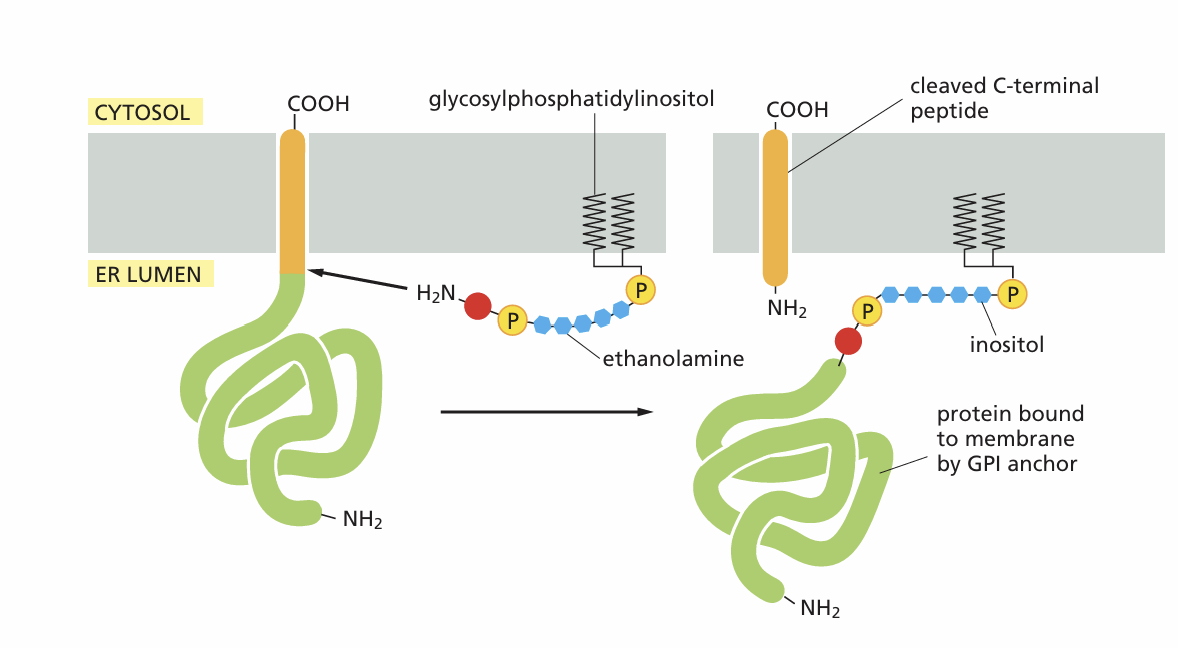
\includegraphics[width=0.5\linewidth]{GPI.png}
    \caption{GPI anchor synthesis}
    \label{fig:enter-label}
\end{figure}

Proteins bound to GPI anchor are translocated to the ER by an \textbf{N-terminal tag that is cleaved off }(not shown in figure). The hydrophobic \textbf{C-terminus remains bound to the membrane}. This is cleaved off and replaced by the \textbf{GPI anchor, which faces into lumen}


\begin{figure}[H]
    \centering
    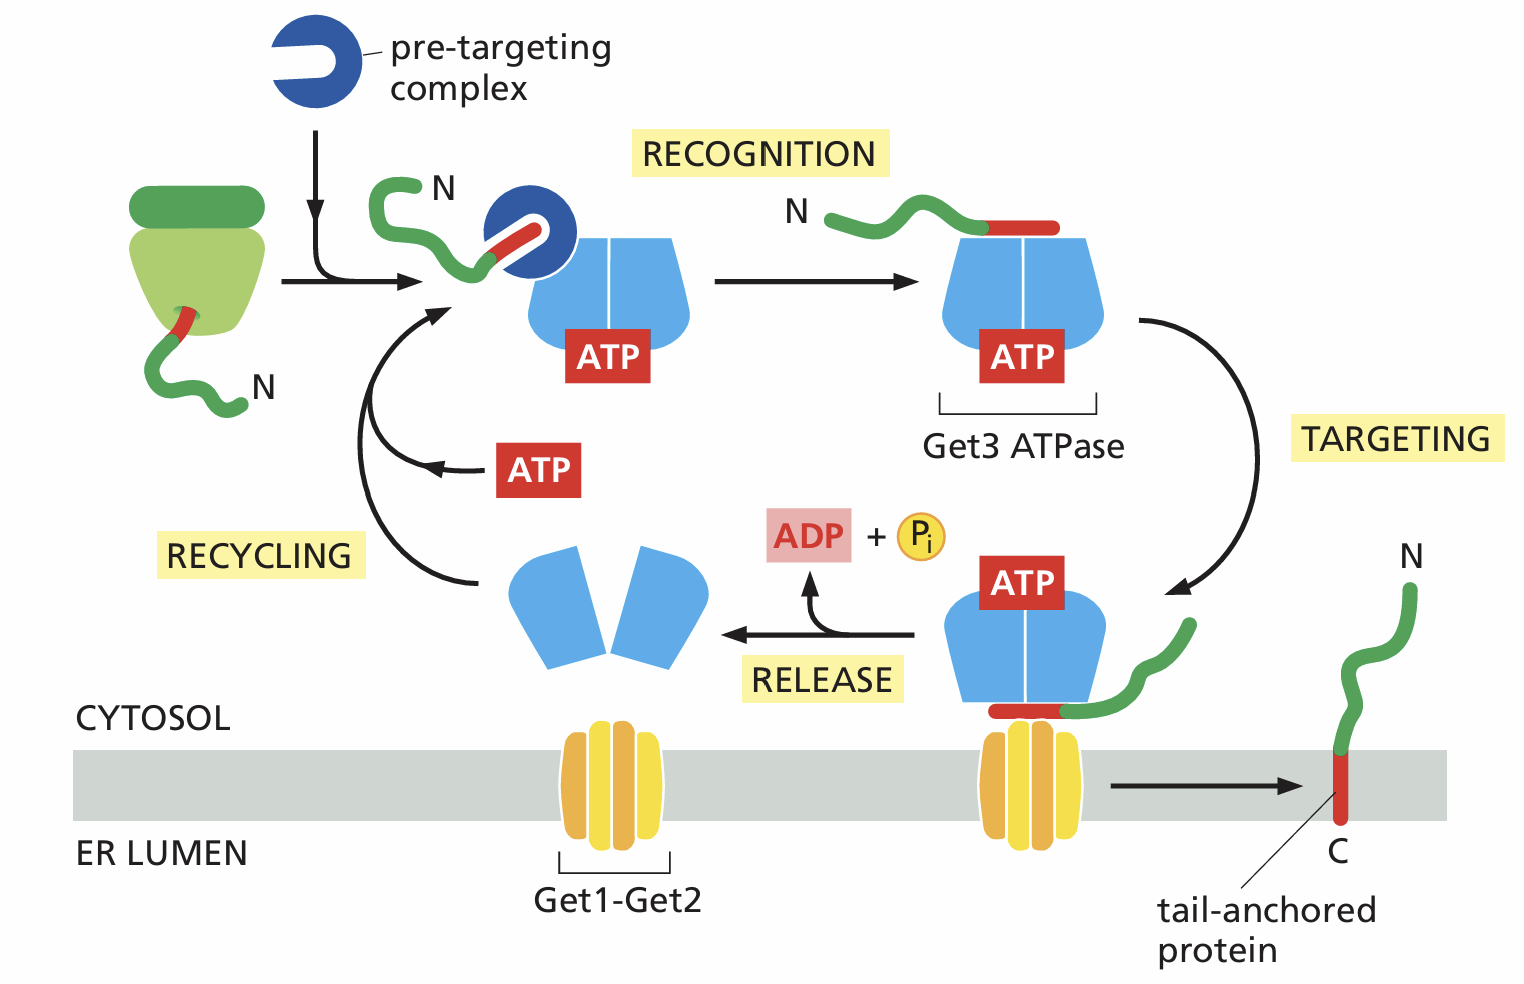
\includegraphics[width=0.5\linewidth]{tailAnchoredProteins.png}
    \caption{tail anchored proteins}
    \label{fig:enter-label}
\end{figure}
Another method of anchoring the protein is directly via the C-terminus. This works as follows:

\begin{enumerate}
    \item tail anchored protein is synthesized in cytosol
    \item \textbf{pre-targeting complex} recognizes the hydrophobic tail of the protein (red segment) and delivers it to\textbf{ \gls{get3}}
    \item the get3-"cargo" complex is handed to get3-ATPase, which will localize to the ER where it will bind to \textbf{get1-get2}
   \item the get1-get2 complex will release the hydrophobic C tail of the protein into the membrane. \textbf{Unlike GPI these face the cytosolic side.}
\end{enumerate}


\paragraph{moving ribosomes to ER: The signal-recognition particle (SRP)}
\begin{figure}[H]
    \centering
    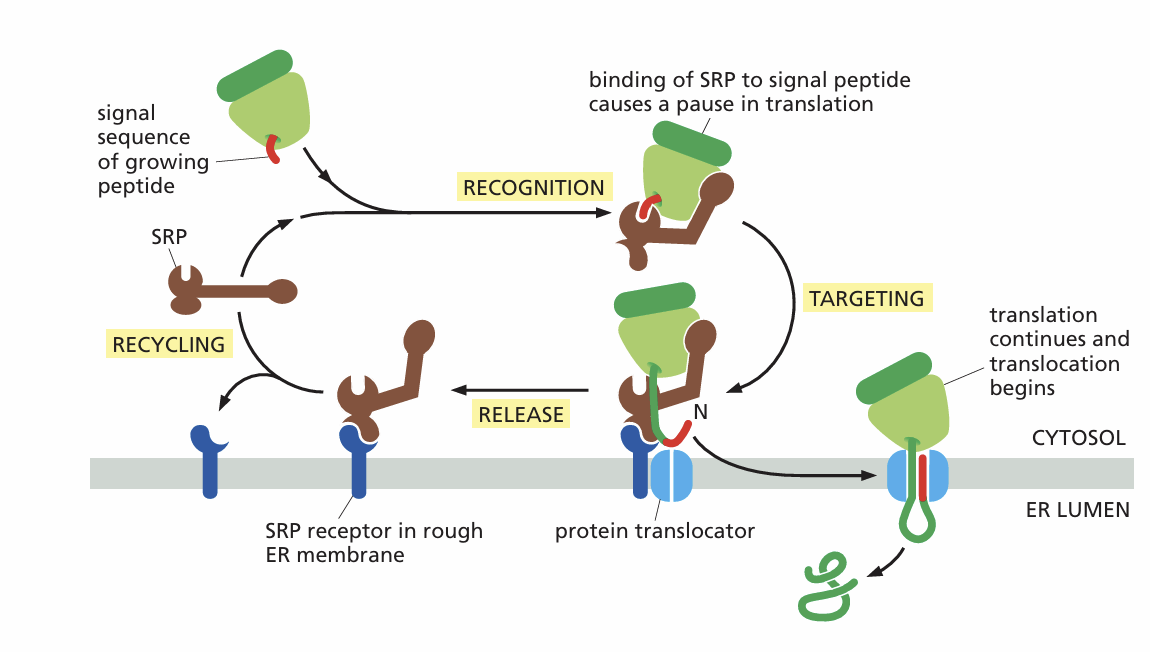
\includegraphics[width=1\linewidth]{SRP.png}
    \caption{The SRP function in ribosome localization}
    \label{fig:enter-label}
\end{figure}
\begin{enumerate}
    \item \textbf{Recognition:} The SRP binds to the signal sequence emerging from the ribosome as the protein is being synthesized. This binding pauses translation.
    
    \item \textbf{Targeting:} The SRP-ribosome complex is directed to the ER membrane, where it binds to the SRP receptor located in the rough ER membrane.
    
    \item \textbf{Release:} The SRP dissociates from the ribosome upon interaction with the SRP receptor, allowing the ribosome to engage with the protein translocator.
    
    \item \textbf{Translocation:} Translation resumes, and the growing polypeptide is threaded through the \gls{translocator} into the ER lumen.
    
    \item \textbf{Recycling:} The SRP is released and recycled for future rounds of protein targeting.
\end{enumerate}




\subsubsection{the role of contact patches in protein transport}
\begin{figure}[H]
    \centering
    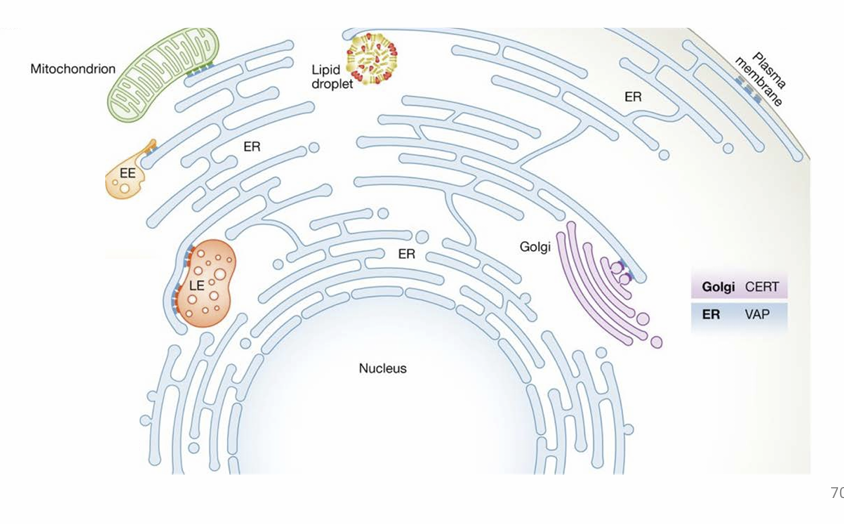
\includegraphics[width=0.5\linewidth]{contact.png}
    \caption{Contact patches role in protein transport}
    \label{fig:enter-label}
\end{figure}
Contact patches are contact points between organelles where certain proteins and lipids can be exchanged. these are not random bumping into eachother kinda thing but \textbf{highly regulated interactions} that are \textbf{new and not well understood}

\subsubsection{topological equivalence principle}
\begin{figure}[H]
    \centering
    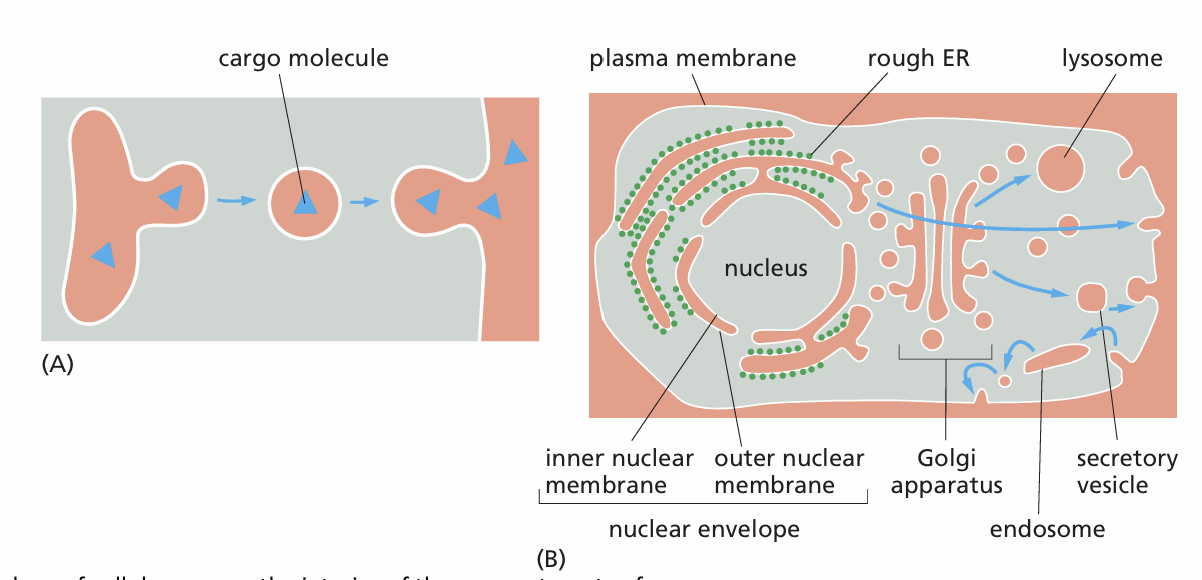
\includegraphics[width=0.5\linewidth]{topologicalEquivalence.png}
    \caption{topological equivalence}
    \label{fig:enter-label}
\end{figure}
The idea of topological equivalence is that the leaflets exposed to the cytosol have similar composition and thus can communicate with eachother. The \textbf{inner compartments of the organelles are equivalent to the extracellular space.} This is a \textbf{concequence of vesicle transport}.
\par
\paragraph{how do luminal proteins and secreted proteins form if ribosomes are cytoplasmic?}
Via the topological equivalence principle, a protein can move via vesicular transport to any other topologically equivalent region. However if a protein is luminal (in the ER lume ect.) It faces the issue that the ribosomes themselves are cytosolic so it could't enter the lumen. THis is\textbf{ solved by cotranslational translocation} where the ribosomes are translocated so they synthesis the protein directly into the ER lumen. \textbf{All proteins that are luminal, membrane or secreted are synthesized by ribosomes attached to ER not free ribosomes}

\paragraph{membrane directionality}
Membrane directionality is also a cause of vesicular transport as for example a luminar leaflet will never point towards the cytosol and vesicule transport only allows transport between topologically equivalent domains. 

\begin{figure}[H]
    \centering
    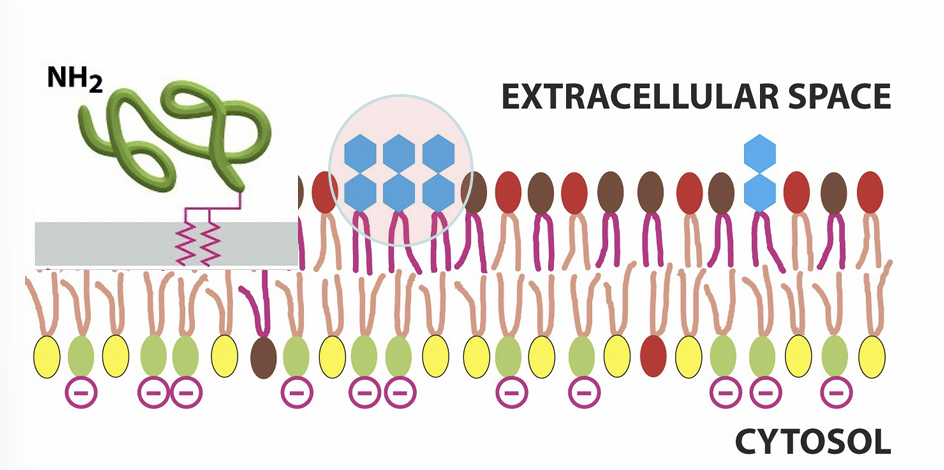
\includegraphics[width=0.7\linewidth]{asymetry.png}
    \caption{Asymetry in membrane leaflets}
    \label{fig:enter-label}
\end{figure}

\subsection{glycosylation}
Glycosylation serves many purposes in the cell some of those being: 
\begin{enumerate}
    \item helps the protein fold 
    \item their presence on the surface of a protein will protect them from extracellular proteases
    \item give information on how long a protein has been around and it's fold status (misfolded or not)

glycosylation occurs in the\textbf{ sequence:  Asn-X-Ser/Th}
\end{enumerate}
\paragraph{N linked glycosylation in ER vs O linked in golgi}
\begin{figure}[H]
    \centering
    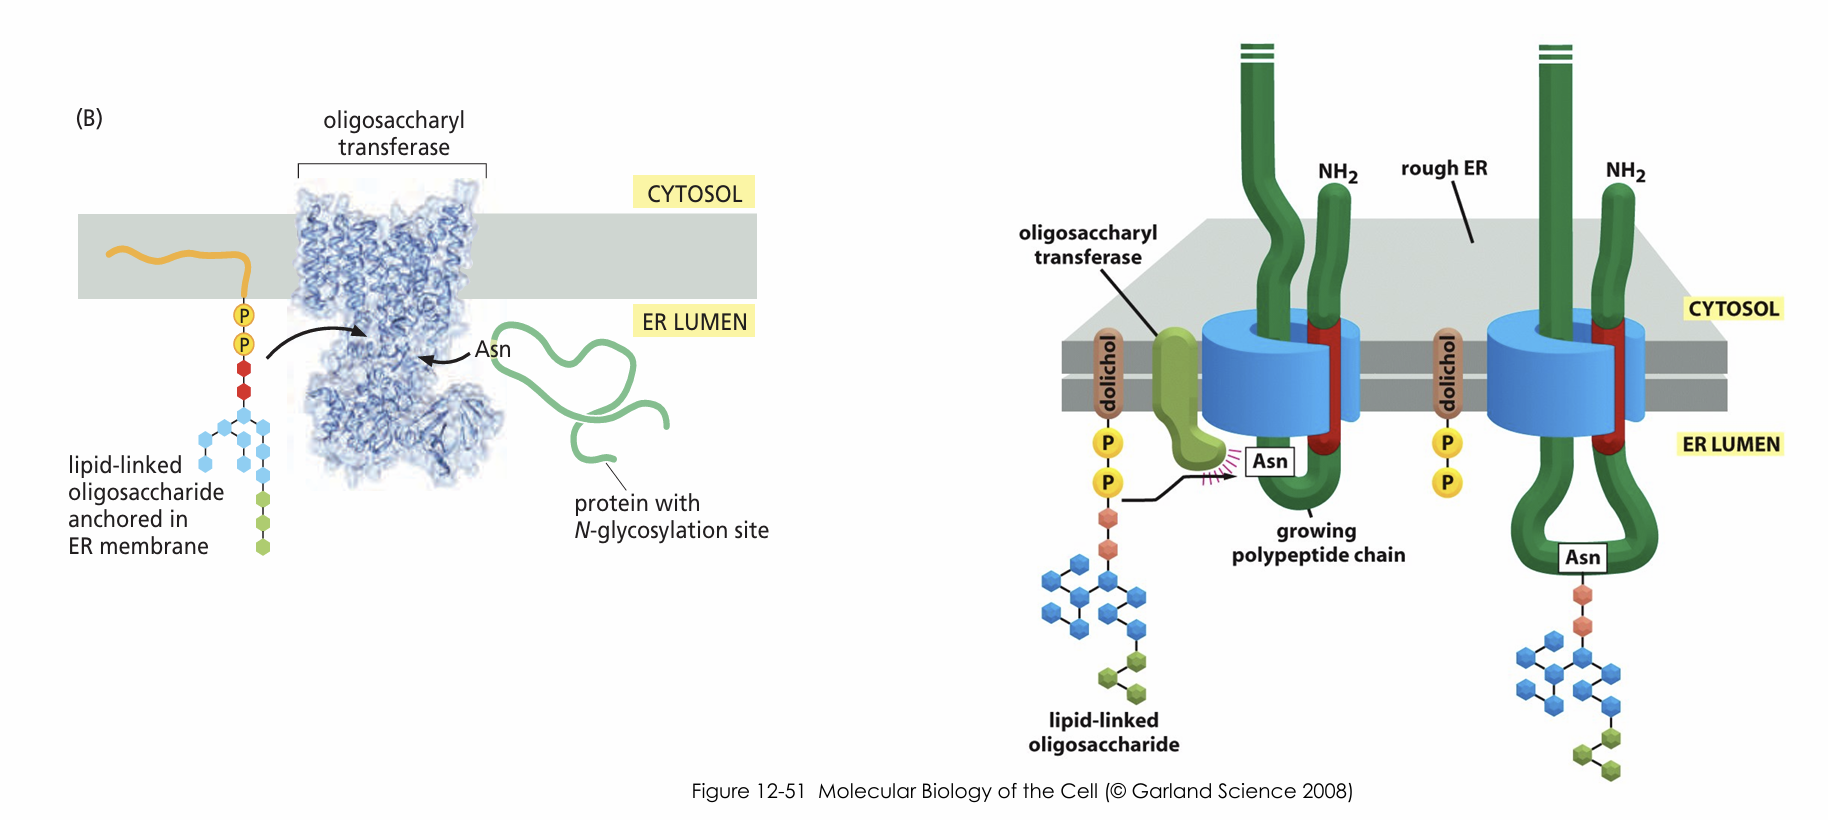
\includegraphics[width=\linewidth]{ERLinkedGlyc.png}
    \caption{ER linked glycosylation}
    \label{fig:enter-label}
\end{figure}

In the ER glycosylation occurs \textbf{all at once.} where the entire "sugar tree" that was built on \gls{diochol} is transfered to the protein as it passes throught the translocator complex.


\subparagraph{N linked glycosylation vs O-linked glycosylation}
\begin{figure}[H]
    \centering
    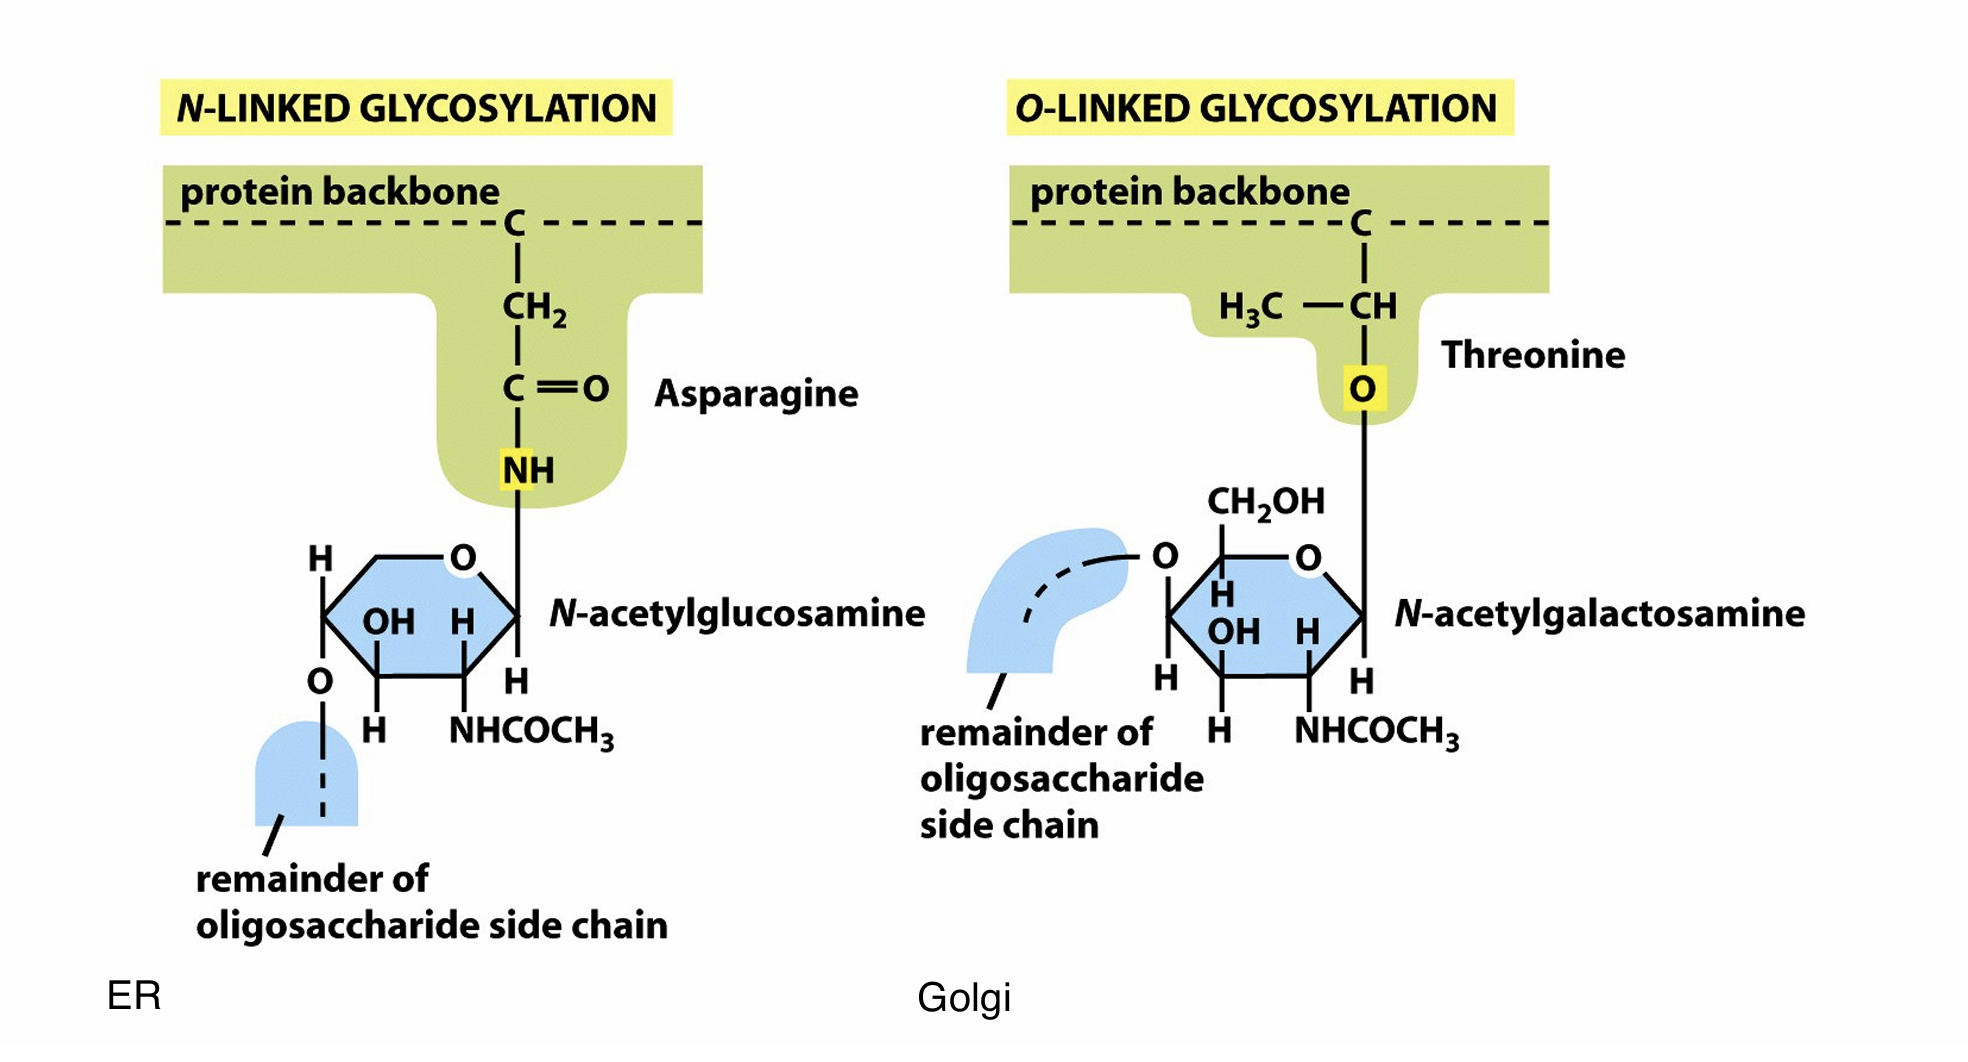
\includegraphics[width=0.7\linewidth]{glycosylation.png}
    \caption{N linked vs O linked glycosylation}
    \label{fig:enter-label}
\end{figure}
There is a slight difference in glycosylation depending on where it is produced. The glycosylation occouring in the \textbf{ER will be N-linked} (i.e on an Oxygen atom) while the glycosylation occuring in the \textbf{golgi will be O-linked (i.e on a Nitrogen atom)}


\paragraph{Calnexin/Calreticulin cycle \& ER protein folding }

\begin{figure}[H]
    \centering
    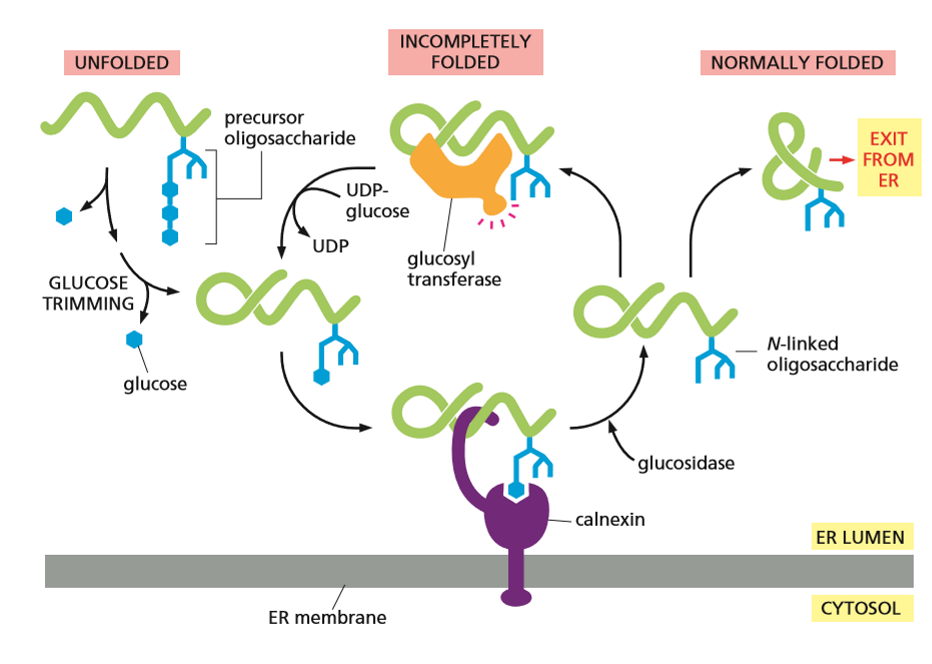
\includegraphics[width=\linewidth]{calCycle.png}
    \caption{\gls{calnexin_cycle} cycle in ER}
    \label{fig:enter-label}
\end{figure}
\textbf{Calnexin and calreticulin} are two chaperones that will \textbf{bind to N-linked sugars}. THis binding then prevents the protein from aggregating before it is fully folded.
\par
 If the protein has completed folding \textbf{\gls{glucosyltransferase}} will add a glucose. At the same time \textbf{\gls{mannosidase}} will \textbf{cleave off mannoses from the sugar tree that was added all at once}. The amount of mannose is thus an indicator of how long the protein has been trying to fold. If it takes to long it will be marked for destruction by addition of \textbf{polyubiquitin }that signals them to be sent to the \textbf{proteosome}.

\subparagraph{The unfolded protein response}
\begin{figure}[H]
    \centering
    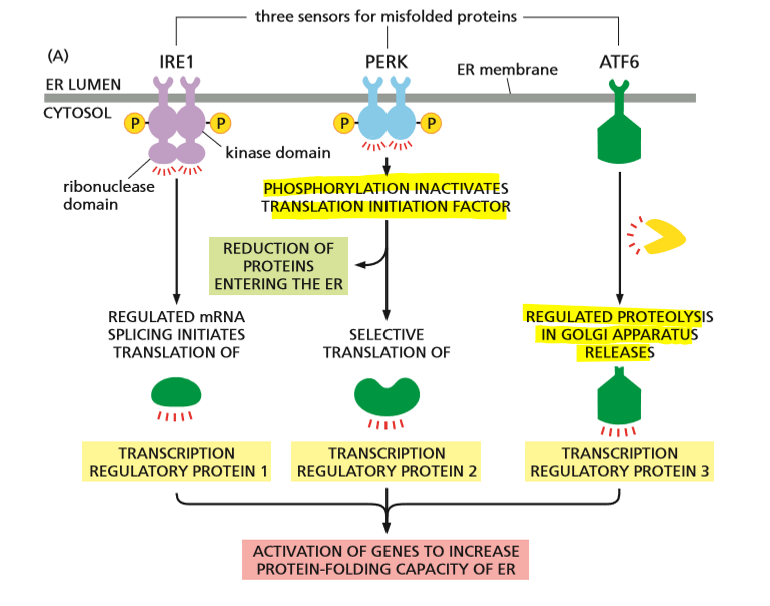
\includegraphics[width=\linewidth]{UnfoldedProteinResponse.png}
    \caption{the unfolded protein response}
    \label{fig:enter-label}
\end{figure}
\begin{enumerate}
    \item Misfolded proteins in ER signal the need for more ER chaperones. They bind to and activate a transmembrane kinase.
    \item Activated kinase unmasks an endoribonuclease activity (domain that cuts RNA).
    \item Endoribonuclease cuts specific RNA molecules at two positions, removing an intron.
    \item Two exons are ligated to form an active mRNA.
    \item mRNA is translated to make a transcription regulator.
    \item Transcription regulator enters nucleus and activates genes encoding ER chaperones.
    \item Chaperones are made in ER, where they help fold proteins.
\end{enumerate}

\subsection{phosphatydilcholine sythesis in Er}
\begin{figure}[H]
    \centering
    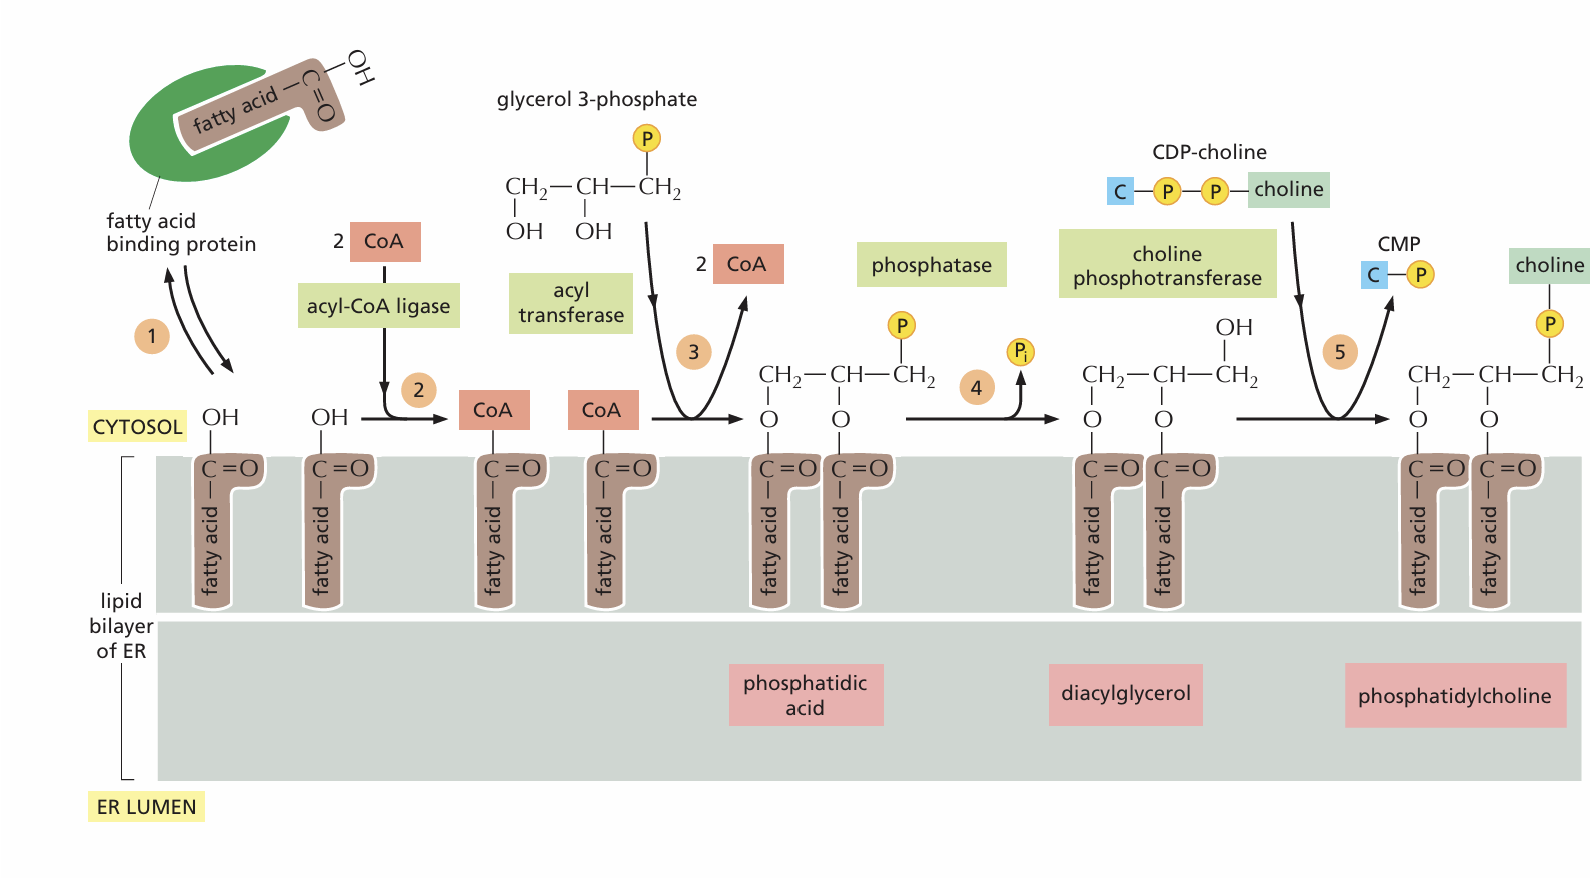
\includegraphics[width=0.5\linewidth]{phosphatydilCholineSynthesis.png}
    \caption{Phosphatydil Choline Sythesis}
    \label{fig:enter-label}
\end{figure}
Phosphatydil choline is sythesized on the \textbf{cytosolic leaflet of the ER}. This would lead to assymetries where there no \textbf{scrablases} to shuffle the lipids between the two leaflets.

\end{document}